
\documentclass{llncs}
\usepackage{graphicx}        % standard LaTeX graphics tool
                             % when including figure files
\usepackage{subfigure}
\usepackage{url}
%%%%%%%%%%%%%%%%%%%%%%%%%%%%%%%%%%%%%%%%%%%%%%%%%%%%%%%%%%%%%%%%%%%%%%%%%%%%%%%%%%%%%%%%%

\begin{document}
\sloppy

\title{Random Selection of Parameters in Asynchronous Pool-Based Evolutionary Algorithms}

\author{Mario Garc\'ia-Valdez\inst{1} 
\and Ren\'e M\'arquez\inst{1} \and Juan J. Merelo Guerv\'os\inst{2} \and  Leonardo Trujillo \inst{1}}

\institute{Instituto Tecnol\'ogico de Tijuana, Tijuana BC, Mexico
\and
Universidad de Granada, Granada, Spain
\email{mario@tectijuana.edu.mx}\\
\email{renemarquezvalenzuela@gmail.com}\\
\email{jmerelo@geneura.ugr.es}\\
\email{leonardo.trujillo@tectijuana.edu.mx}}

\maketitle

\begin{abstract}
It is not always possible to set up an distributed system with
homogeneous nodes to run algorithms in a synchronous way. In grid,
cloud or volunteer setups nodes are heterogeneous, or simply are not
available at the exact same time; this is a challenge for the researcher if
their full performance is going to be actually leveraged. We are
interested in evolutionary algorithms (EAs), which evolve a population
of solutions using a mechanism inspired by biological evolution; in this field, 
several asynchronous Evolutionary Algorithms (EAs) that distribute the
evolutionary process among heterogeneous nodes have
been proposed. These algorithms make the population shared between
distributed workers  which execute the actual evolutionary
process by taking samples of the population, and replacing them in the
population pool by evolved individuals. The performance of these EAs
depends in part on the selection of parameters for the EA running in
each worker, which may include sample size, generations, mutation rate
and crossover rate along with the overall configuration. In this paper
we present a method inspired by a strategy proposed by Gong and Fukunaga for the
Island-Model which statically assigns random parameter settings to
each island in a cloud setting. Experiments were conducted in the
cloud using 2, 6 and 12 virtual machine configurations, with
both homogeneous and heterogeneous random settings using five 
test functions for single-objective optimization (Rastrigin, Griewank, De Jong, Schaffer 
and Ackley) and the OneMax binary problem. The results suggest that this approach can yield
performance improvements which are competitive with instances of the
algorithm using workers with control parameters tuned specifically for
the benchmark.

% Abstract proposed by Leonardo
% This work studies pool-based evolutionary algorithms (PEAs), that
% asynchronously distribute the evolutionary process among multiple computing nodes.
% PEAs provide a central repository or pool where the complete population is stored.
% Distributed nodes (or workers) asynchronously interact with the pool by taking a 
% sample of the population and performing a local evolutionary search on the population
% sample, then returning to the pool the newly evolved solutions.
    %%% Not all PEAs here you are talking about EvoSpace, others
    %%% you can have an island model using PEAs, and migration is throu the pool - Mario  
% Like any other EAs, the performance of the complete search will depend
% on the correct tuning of the EA parameters. In this case this problem 
% is magnified by a factor of $N$, the number of workers.
% This paper evaluates two approaches. First, to set the main parameters 
% homogeneously across all workers, based on a previous random sampling of parameter space.
% The second approach is based on the work by Gong and Fukunaga 
% proposed for the Island-Model EA called Randomized Parameter Setting Strategy,
% where parameters are set randomly for each worker and are thus heterogeneous across workers.
% Experiments were conducted in the cloud using 2, 6 and 12 virtual machine configurations, using five 
% test functions for single-objective real-valued optimization problems (Rastrigin, Griewank, De Jong, Schaffer 
% and Ackley) and the OneMax binary problem. The results suggest that the heterogeneous approach can yield
% performance improvements over the homogeneous method without requiring any previous tuning heuristic.

\keywords{Distributed Evolutionary Algorithms, Volunteer Computing,
  Cloud Computing}
\end{abstract}
\section{Introduction}

%Why Paralel
Biological evolution is an intrinsically parallel, distributed and asynchronous process, however, 
some of these features are not trivially included into standard EAs,  which are mostly coded as sequential 
and synchronous algorithms \cite{eiben};  a large body of work exists in EA parallelization, 
using multiple CPU cores, multiple nodes and GPUs \cite{cantu2000efficient}.
However, distributed and asynchronous EAs have started to become common only recently. In an effort to
exploit computing resources available from personal computers,
smartphones and tablets as massive data centers there have been many
researchers and companies that have tried to tap them. 
These resources are easily accessible through popular Internet technologies, such as cloud computing, 
peer-to-peer (P2P), and web environments. Moreover, these technologies are intended for the development 
of parallel, distributed and asynchronous systems, such that an EA developed on top of them could easily 
reap the benefits of these features.

%Pool Based
In this work, we are interested in EAs systems that follow a
pool-based approach, where the search process is conducted by a
collection of possibly heterogeneous processes that collaborate using
a shared repository or population pool. We will refer to such
algorithms as Pool-based EAs or PEAs, and highlight the fact that such
systems are intrinsically parallel, distributed and asynchronous.
The particular PEA implemented in this paper is implemented on 
the EvoSpace framework  \cite{GValdez2015}
in which distributed nodes (or workers) asynchronously interact 
with the pool by taking a sample of the population and performing 
a local evolutionary search on the population sample, then returning 
to the pool the newly evolved solutions. 
% EA Paramaters 
Like any other EAs, the performance of the complete search will depend
on the correct tuning of the EA parameters. However, settings 
must be optimized to each particular problem \cite{de2007parameter}  
giving users an additional optimization task. 
Substantial work has focused on facilitating the burden of finding 
the most appropriate parameters settings, suggesting several strategies:
using parameters of previous studies \cite{eiben1999parameter} 
optimization by another genetic algorithm \cite{grefenstette1986optimization}, dynamic adaptation \cite{eiben1999parameter}, 
self-adaptive parameters \cite{pellerin2004self}, hybrid approaches and so on.
% Worst on many workers
In heterogeneous and distributed PEAs like EvoSpace, this problem can 
be magnified by a factor of $N$, the number of workers, because each one
can be treated as an independent EA with local parameters. Moreover, there
are additional parameters particular to the EvoSpace framework, 
for instance the size of the samples.
% Dynamic adaptation
Several works propose the use of adaptive crossover and mutation probabilities
that depend on the current genetic diversity of the population \cite{pellerin2004self},
arguing that modifying these parameters can prevent the rapid convergence of the 
algorithm. 
% Explore and Exploit 
% Is this pertinent?
A common dynamic heuristic is to explore the solution space first and then exploit
when a local optima is found and repeat if necessary.  
% Random Patameters
Having multiple EAs running in parallel with different parameters could be 
equivalent to performing a dynamic adaptation, having some workers exploring
and others exploiting at the same time. 
% Evaluate in EvoSpace
In the study presented here, a recent approach called Randomized Parameter
Setting Strategy (RPSS) \cite{fuku1,fuku2} is applied to EvoSpace and tested on 
several benchmark problems, extending the work presented in \cite{garcia2014randomized} 
in which only trap functions were applied.
The idea behind RPSS is that in a distributed EA, parametrization may be
completely skipped for a successful search, with research showing that when the 
number of distributed process is large enough, algorithm parameters can be set 
randomly and still achieve good overall results. However, work on RPSS has 
only focused on the well-known Island Model for EAs, a distributed but synchronous system.

The remainder of the paper proceeds as follows.  Section \ref{sec:work} 
reviews related work. Afterwards, Section \ref{sec:evo} briefly describes the
proposed EvoSpace cloud implementation, the experimental work is presented in 
Section \ref{sec:experiments}. Finally, a summary and concluding remarks are in
Section \ref{sec:conclusions}.

\section{Related Work}
\label{sec:work}
There are two important practical issues faced by many EA systems, namely the size of the parameter 
space and the high computational cost when it is compared with mathematical programming or numerical techniques.
Concerning the latter, one approach to mitigate this issue is to use parallel or 
distributed implementations \cite{cantu-paz:migration-policies,duda2013gpu}.
For instance, Fern\'andez et al. \cite{nc}% articulo Paco, Gustavo y Leo publucado en Natural Computing}
uses the well-known Berkeley Open Infrastructure for Network Computing (BOINC) to distribute EA runs across a
heterogeneous network of volunteer computers using virtual machines. Another recent example is 
found in the FlexGP system developed by Sherry et al. \cite{sherry2012flex}. FlexGP is probably the first large scale GP system 
that runs on the cloud, using an Island model approach and implemented over Amazon EC2 with a 
socket-based client-server architecture.

Another approach to distributed EAs is the so called pool-based architecture. In general, a 
pool-based system employs a central repository (real or virtual) where the evolving population is stored.
Distributed clients interact with the pool, performing some or all of the basic EA processes 
(selection, genetic operators, survival). A representative work of this approach 
is that by Merelo et al. \cite{agajaj} implementing a JavaScript based PEA that distributes 
the evolutionary process over the web, providing the added advantage of not requiring the 
installation of additional software in each computing node.  Other similar cloud-based solutions 
are based on a global queue of tasks and a Map-Reduce implementation which normally handles failures 
by the re-execution of  tasks \cite{fazenda2012,di2013towards,FlexGP}. Using the BOINC 
volunteer platform  Smaoui et al. \cite{FekiNG09} uses work units that consist of a fitness 
evaluation task and multiple replicas  were produced and sent to different clients.

While using a distributed framework can ease the computational cost, it can also exacerbate the first issue mentioned above;
i.e., it increases the size of the algorithm parameter space, which makes parameter tuning a more difficult task.
The issue of optimal parametrization of EAs is a widely studied subject \cite{de2007parameter}, 
with many approaches in literature. For instance, one of the most successful approaches 
is the F-Racing and iterative F-Racing techniques \cite{lopez2011irace}. 
However, while such algorithms can find high performance parametrizations, 
they require additional computational effort which can be too expensive in some applications
(even if they are more efficient than an exhaustive search).

This paper is inspired by the approach proposed by Gong and Fukunaga
called Randomized Parameter Setting Strategy (RPSS)
\cite{fuku1,fuku2}. 
Originally proposed for an Island Model EA, RPSS sets the parameter values of each subpopulation randomly, 
without any kind of tuning or self-adaptive process. The RPSS approach is to set the parameters 
of each subpopulation randomly at the beginning of the run, a very simple strategy.
Even so, results reported in \cite{fuku1,fuku2} exhibit promise, achieving competitive results 
while substantially reducing the amount of effort required to tune the system.

In a first study, \cite{garcia2014randomized} reported that in effect RPSS 
can be successfully applied to a PEA. However, in that work the
approach was only tested on the P-Peaks generator of multimodal problems proposed by De Jong et al. \cite{Jong:PS97}.
While the problem is theoretically interesting, it can be limited in scope given its reliance on a bit string representation.
Therefore, this work extends the study considering another binary representation problem (OneMax) as well as 
five high-dimensional real-valued optimization benchmarks. Our goal is
to test how general is this approach by considering a different search
spaces and different forms of fitness landscapes. 

% Dynamic adaptation
% Random Patameters

\begin{table}[!t]
\caption{Valid ranges for each EvoWorker parameters. One Max}
\label{tab:params}
\centering
\begin{tabular}{|l|c|c|c|c|c|c| }
\hline
\textbf{Parameter} & \multicolumn{3}{|c|}{OneMax} & \multicolumn{3}{|c|}{Test Functions} \\
\hline
Number of Workers & 2 & 6 & 12 & 2 & 6 & 12\\
\hline
\hline
Population Size & 200 & 280 & 620 & 120 & 150 & 150\\
\hline
Sample Size & 40 & 40 & 40 & 40 & 20 & 10\\
\hline
Maximum Samples & 30 & 40 & 40 & 200 & 100 & 50\\
\hline
Local Generations & 30 & 30 & 30 & 100 & 100 & 100\\
\hline
\end{tabular}
\end{table}

\begin{figure*}[h!t]
    \centering
    \subfigure [2 workers]
    {
        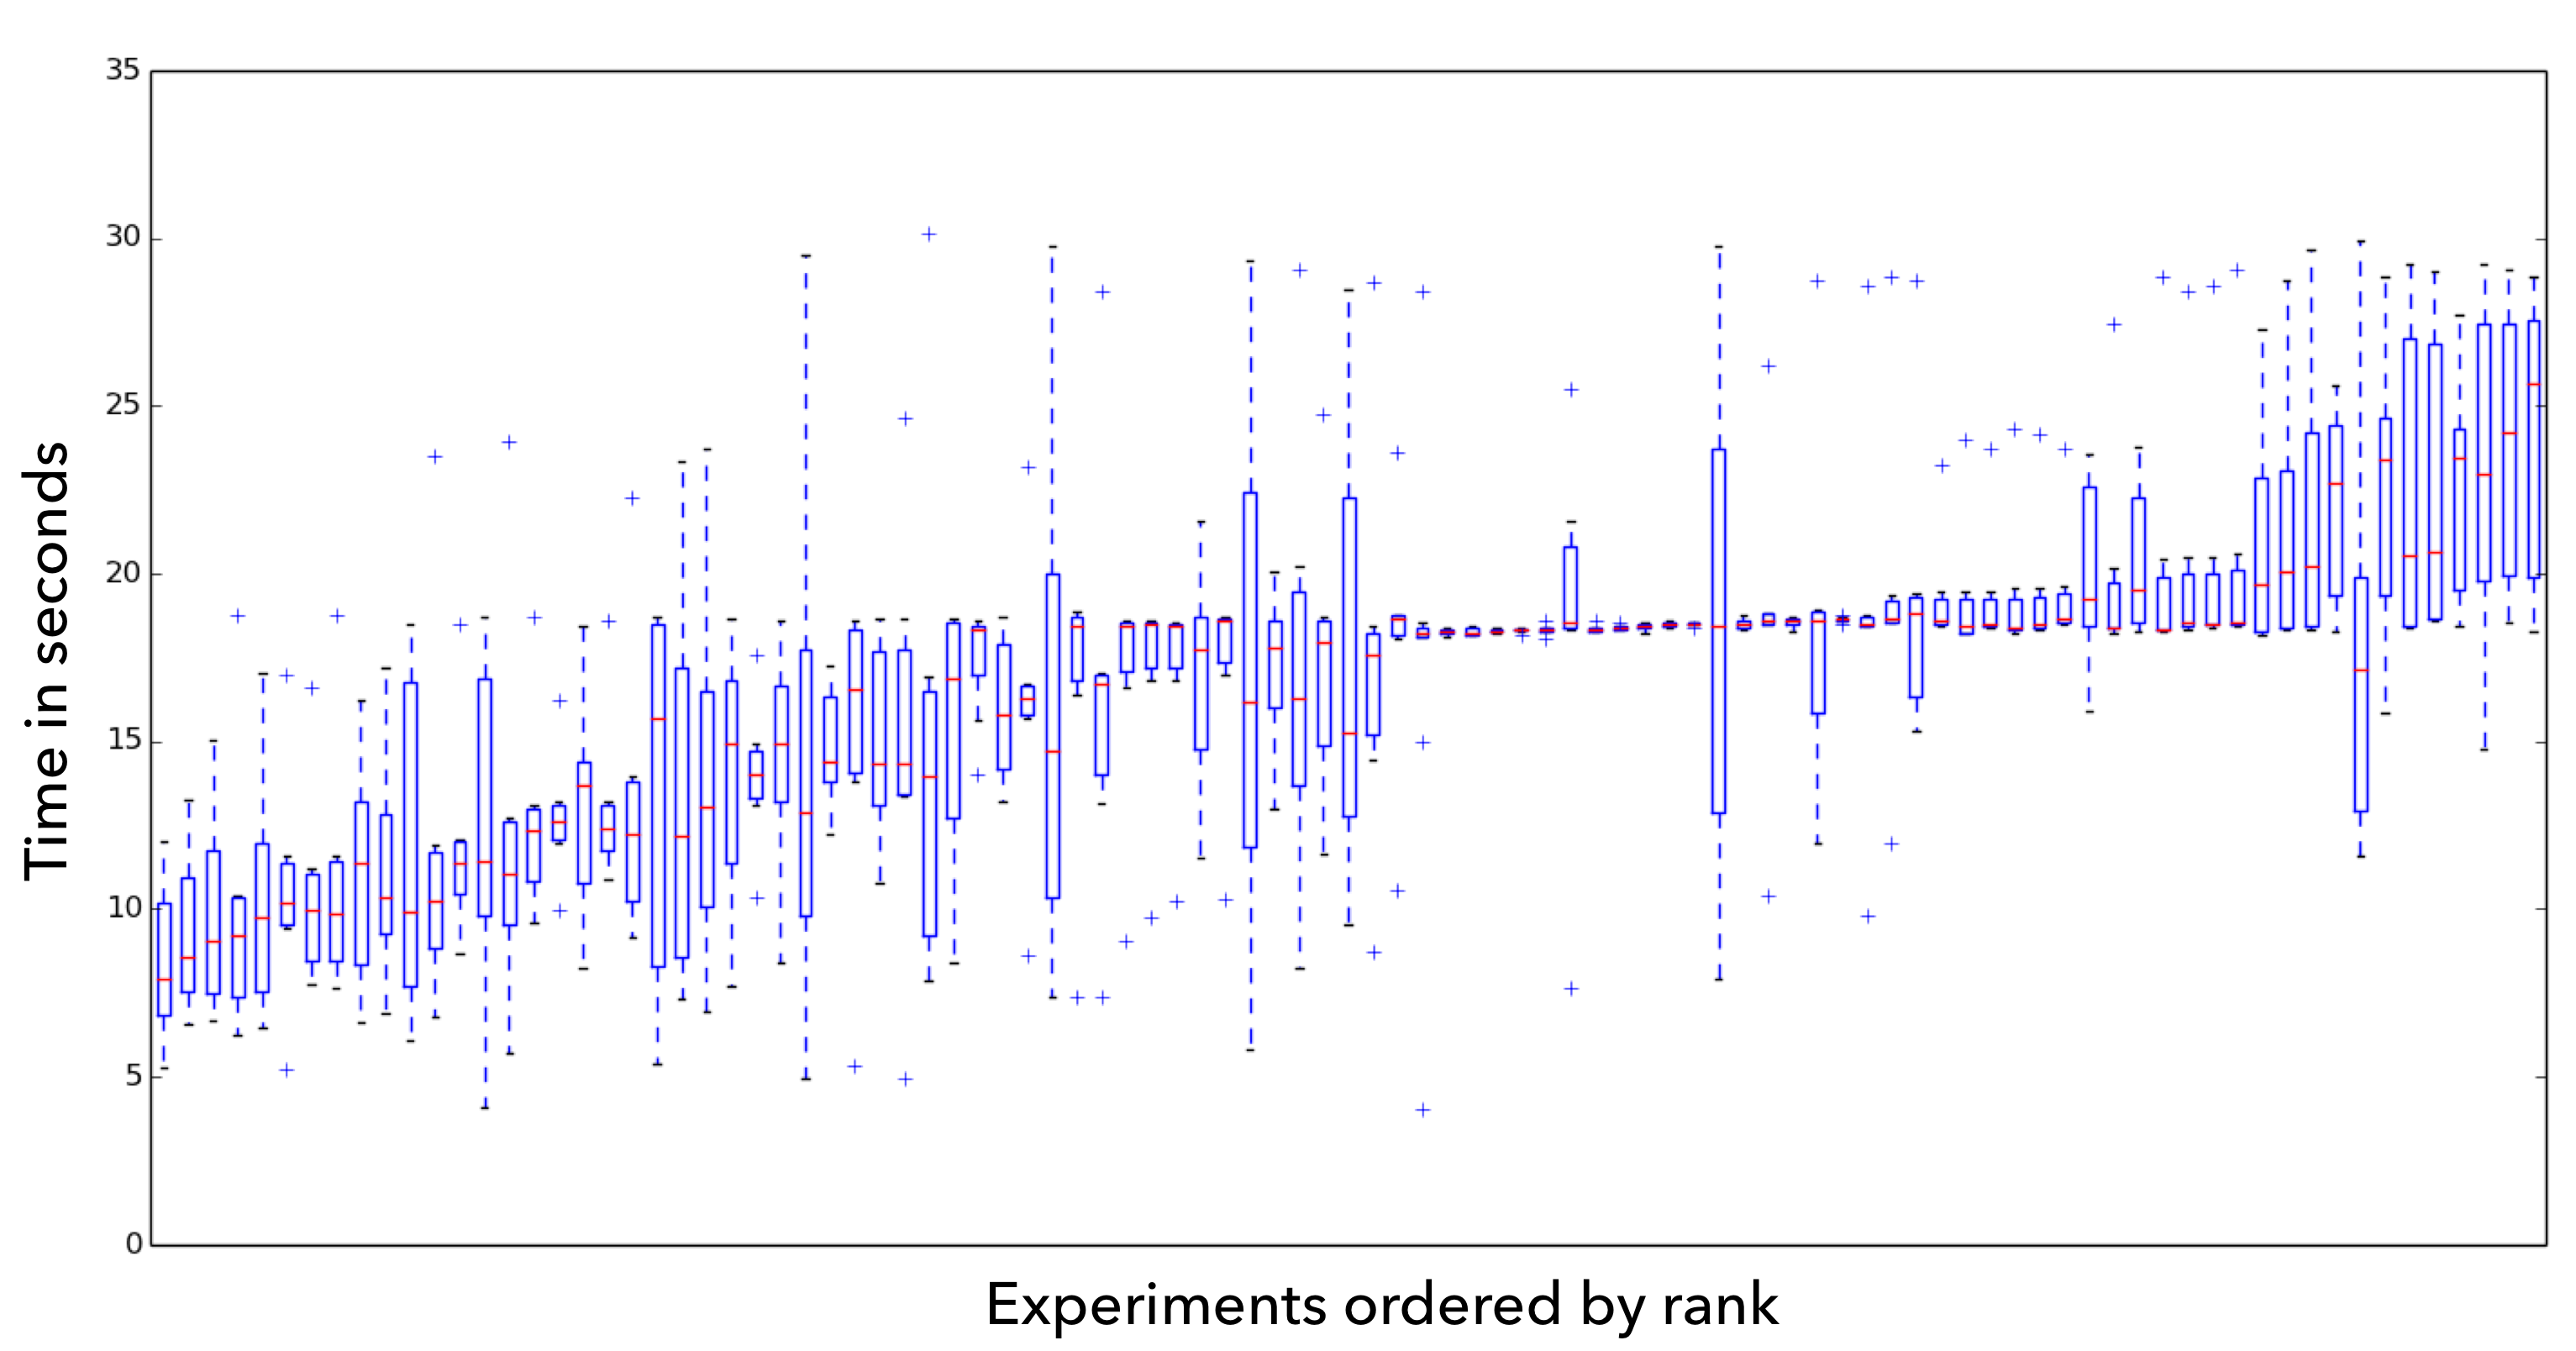
\includegraphics[width=3in]{img/2w_onemax_100_box.png}
    }
    \subfigure  [6 workers]
    {
        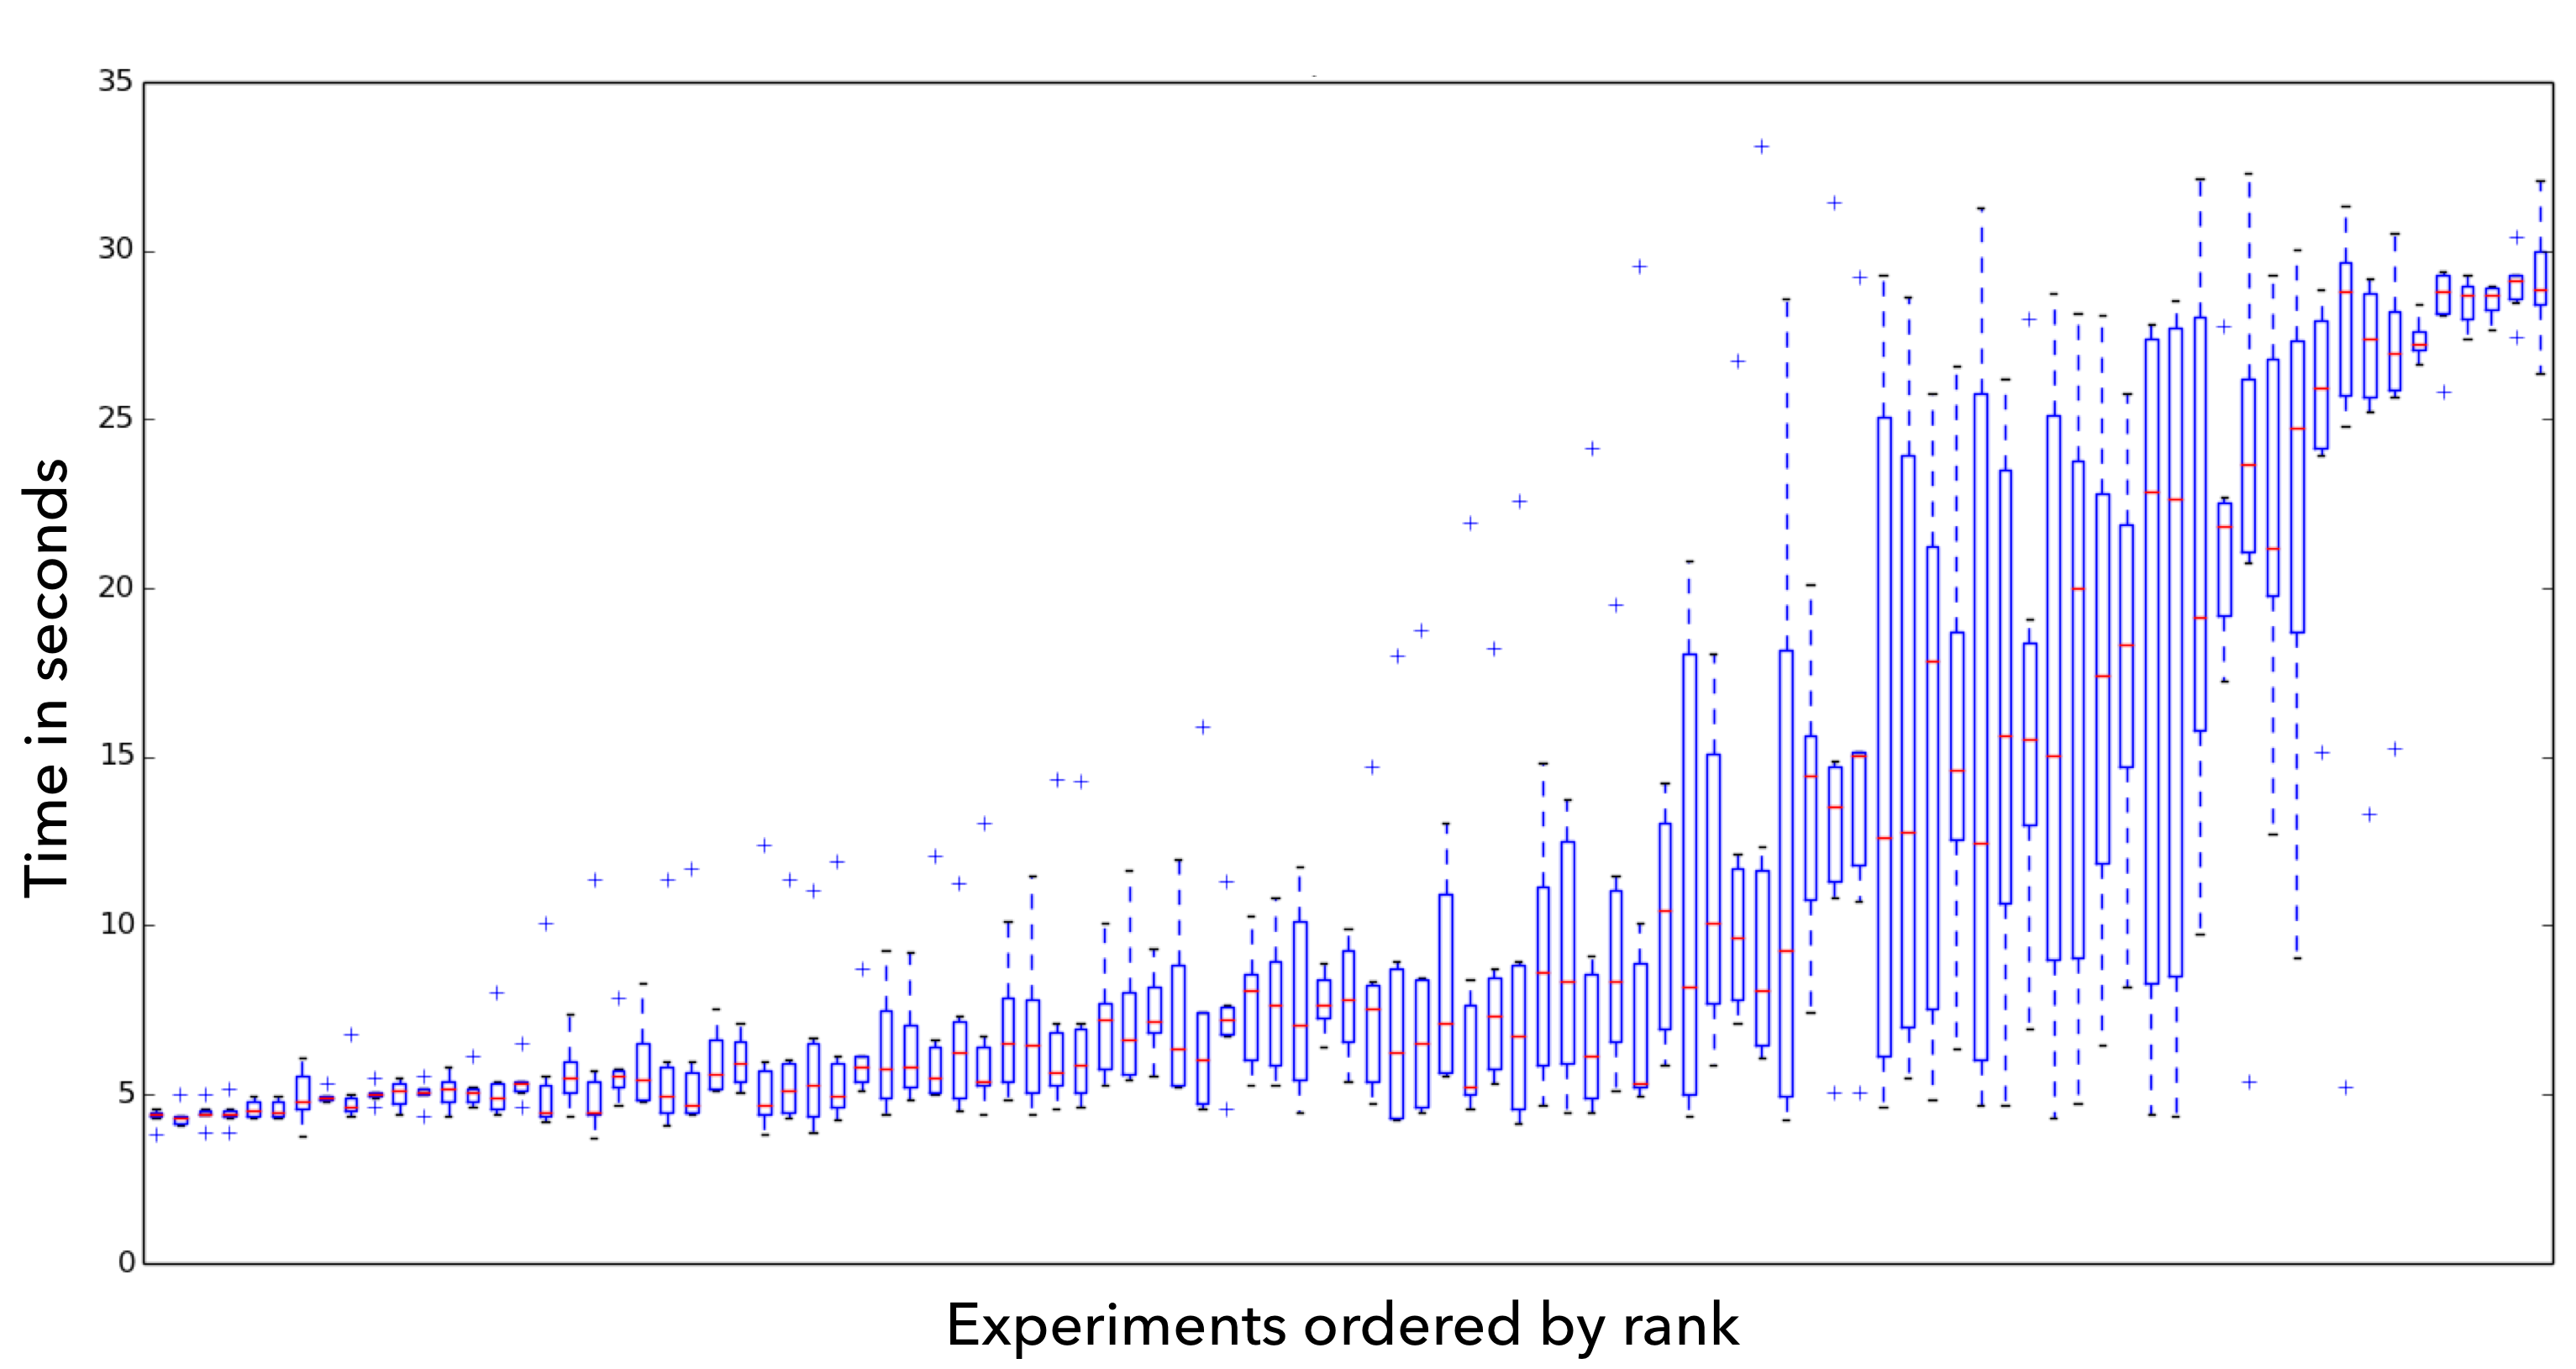
\includegraphics[width=3in]{img/6w_onemax_100_box.png}
    }
    \subfigure  [12 workers]
    {
        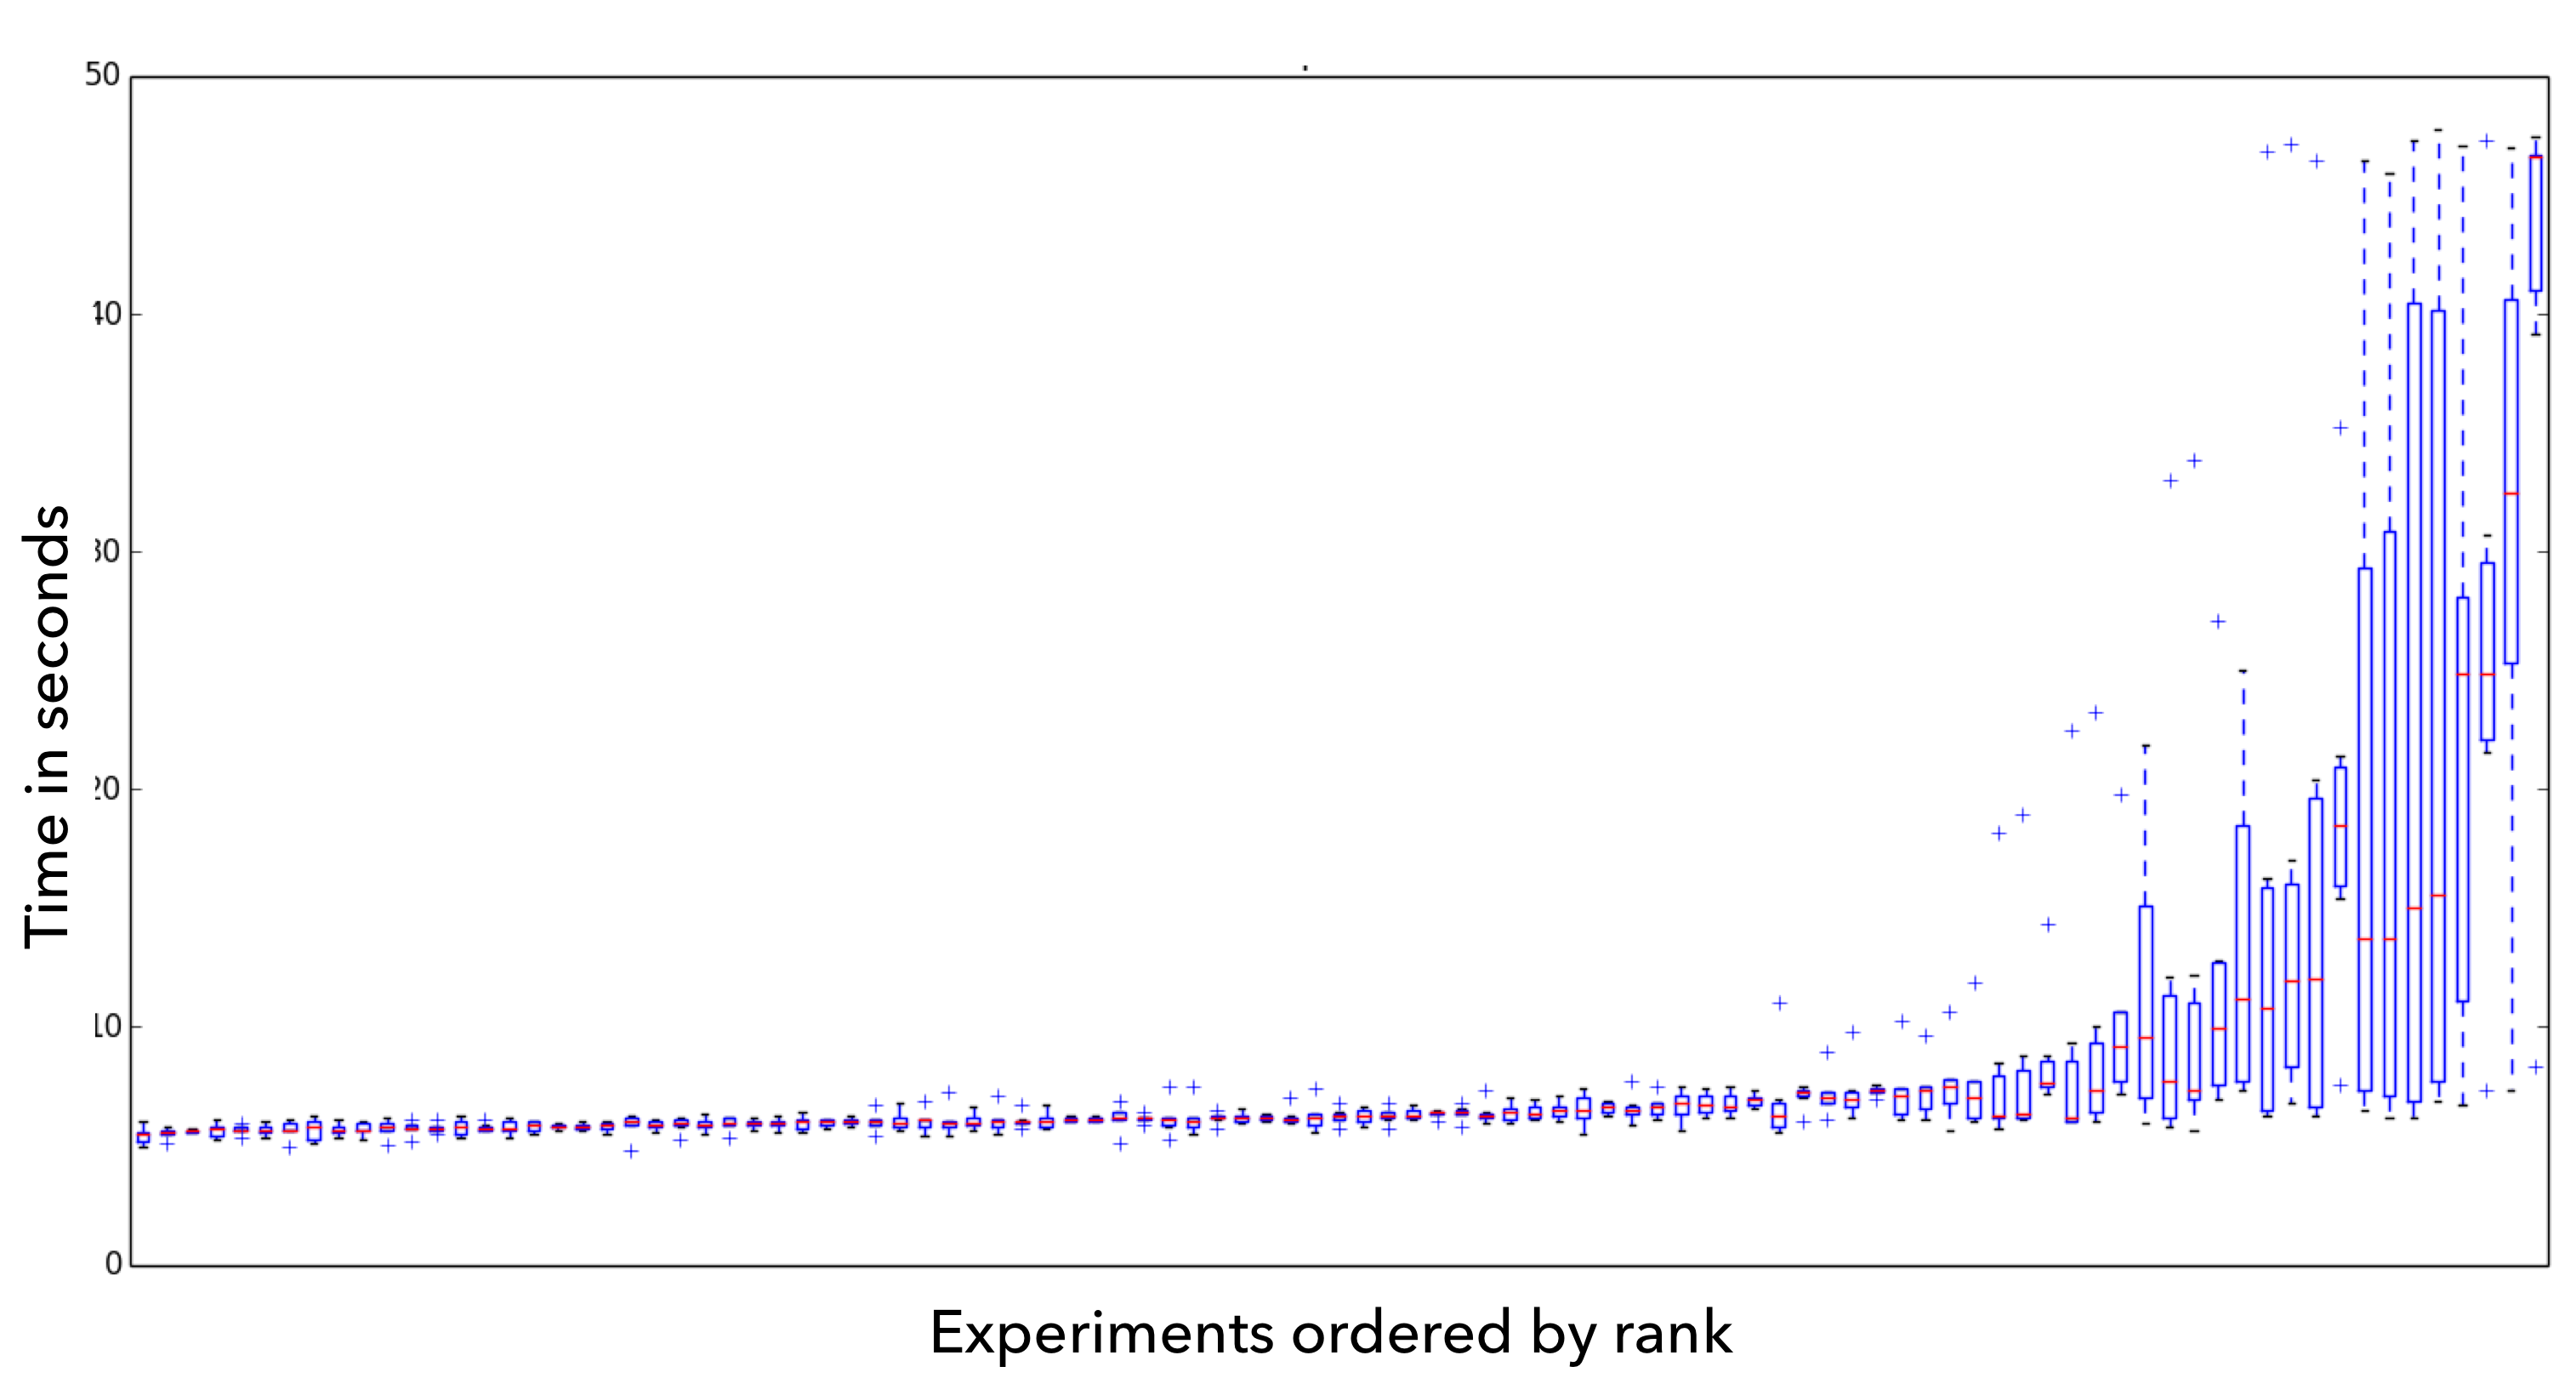
\includegraphics[width=3in]{img/12w_onemax_100_box.png}
    }

    \caption{100 experiments with random parameters for the 128 Bit OneMax problem.
    Experiments are ranked by the mean time to solution of 5 runs, with   
    (a) 2 workers, (b) 6 workers, and (c) 12 workers.}
    \label{fig:effort}
\end{figure*}


\section{EvoSpace Cloud Implementation}
\label{sec:evo}

\begin{figure*}[t]
    \centering
        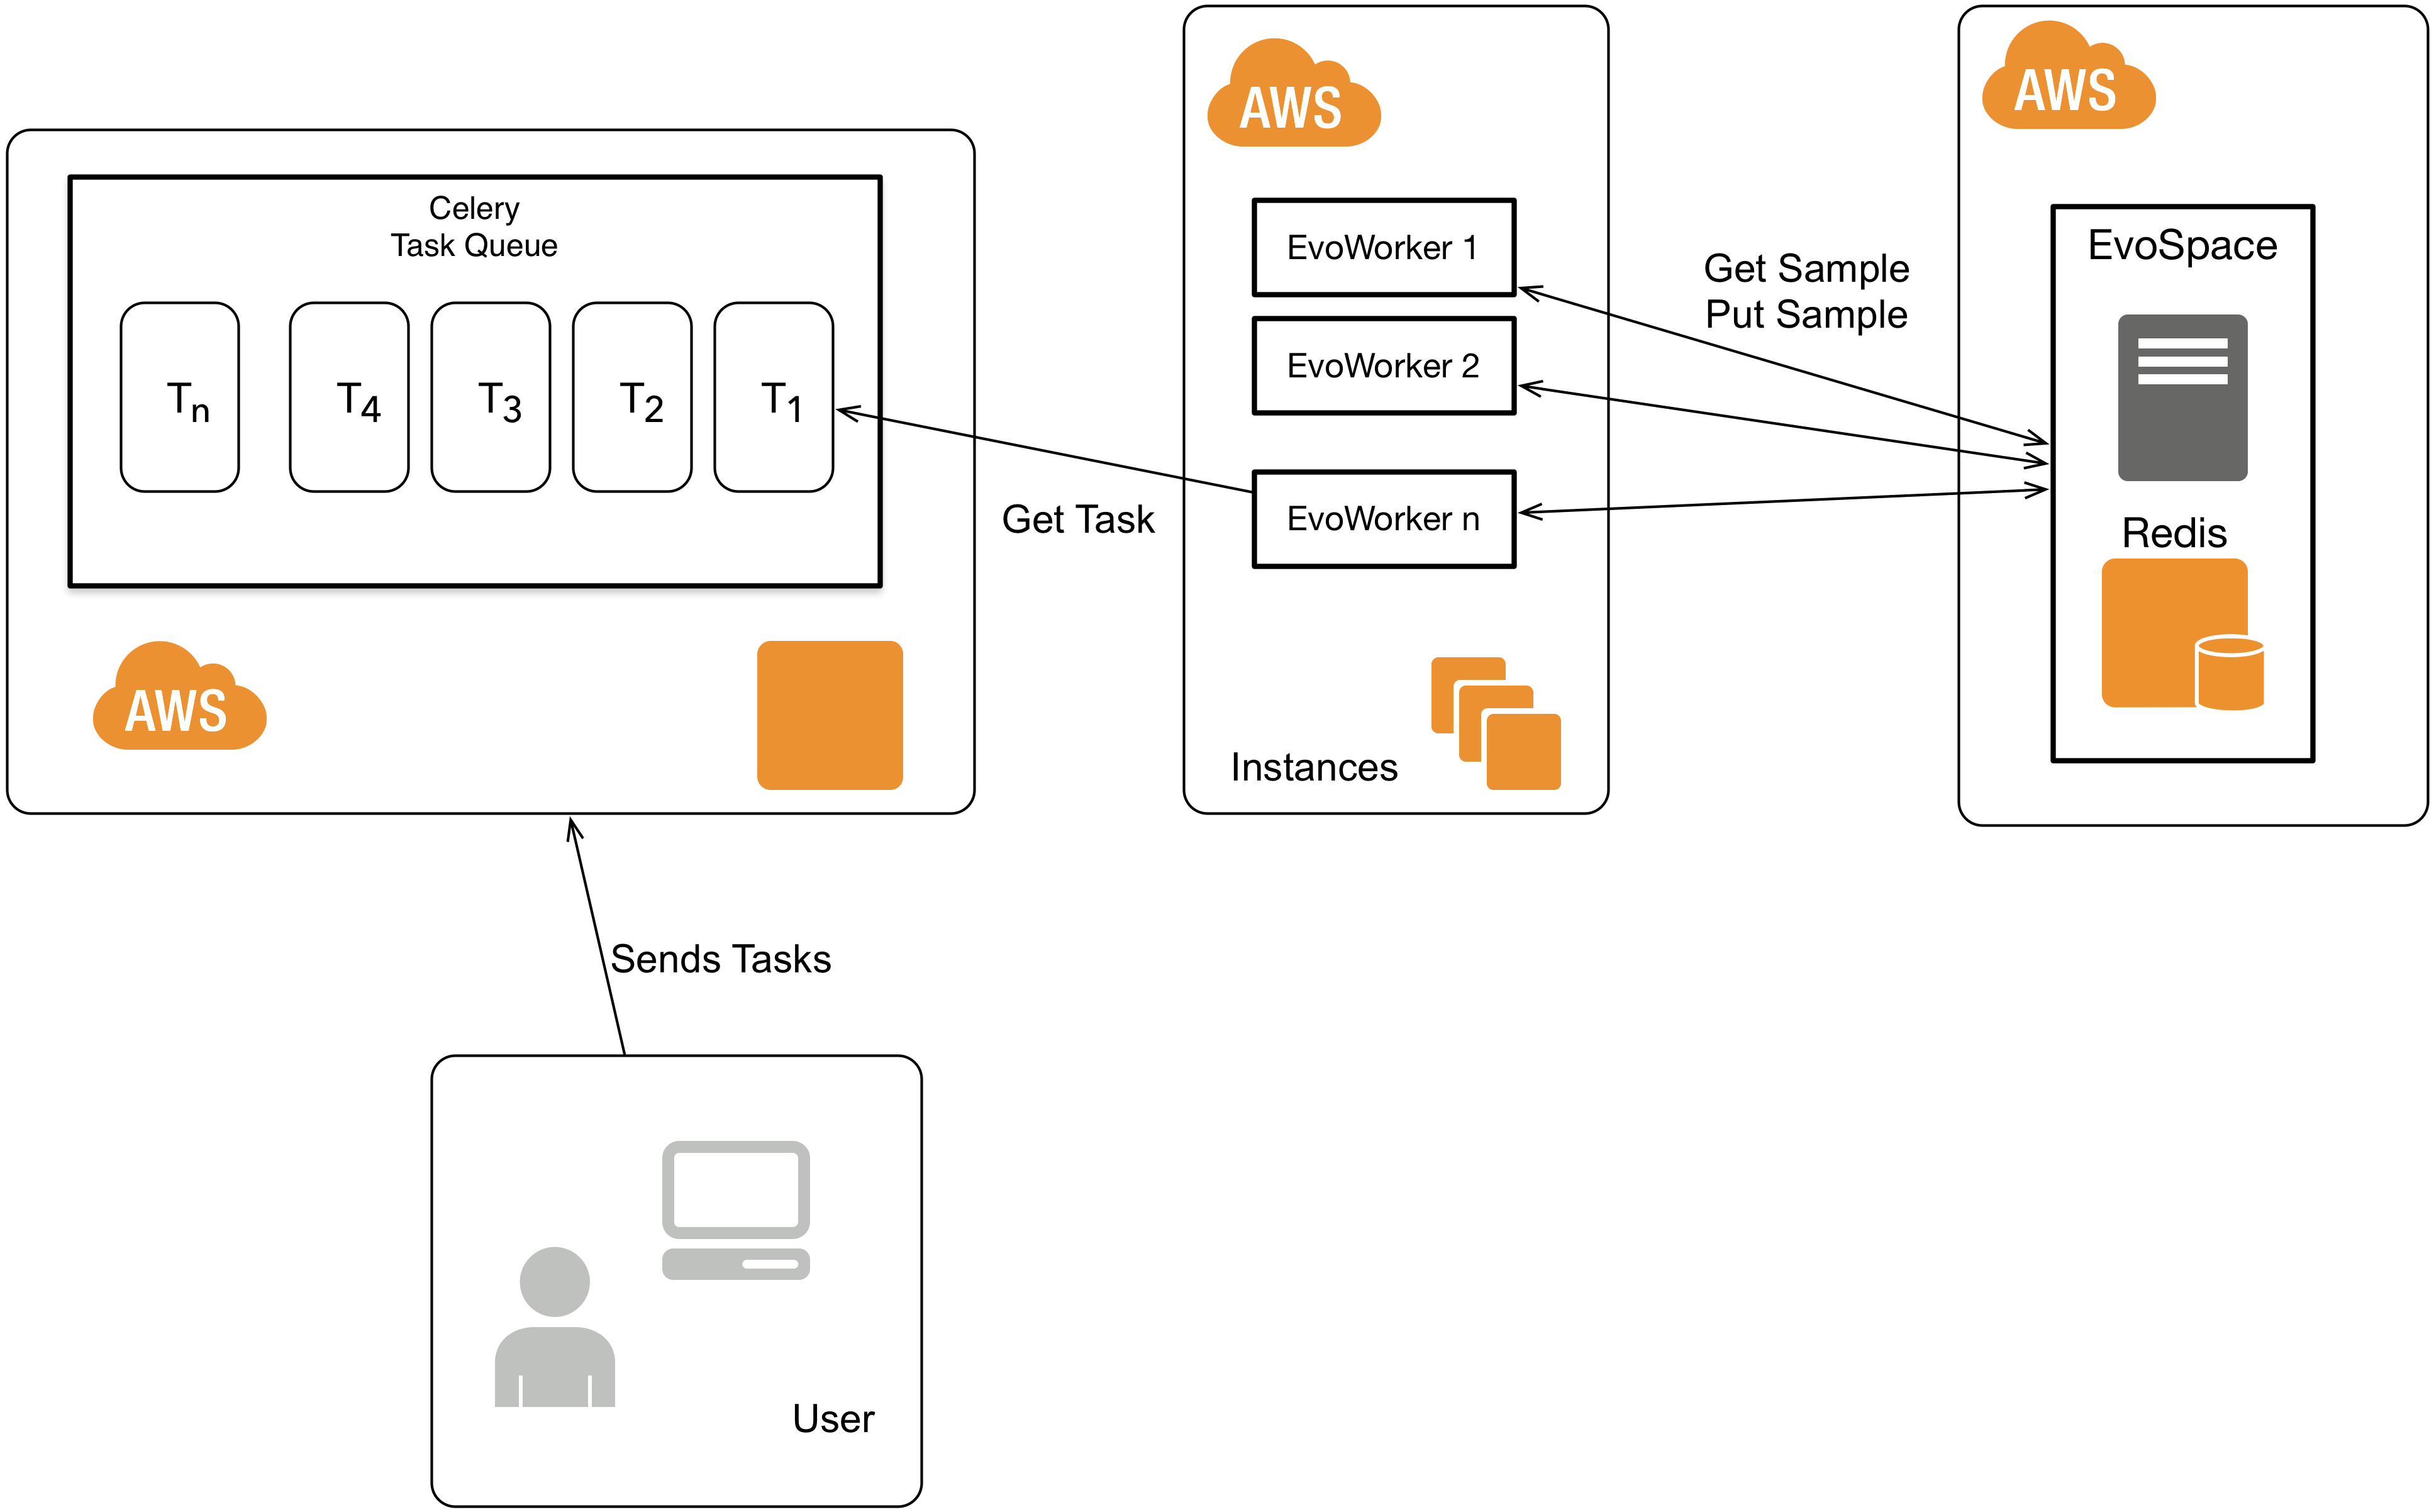
\includegraphics[width=10cm]{img/EvoSpaceAWS.png}
    \caption{Main components and data-flow in the cloud version of EvoSpace. }
    \label{fig:evospace}
  \end{figure*}
  %
The EvoSpace \cite{GValdez2015} framework has two components: (i) the EvoSpace 
container that stores the evolving population and (ii) workers, which execute 
the actual evolutionary process, while EvoSpace container acts only as a population repository.
In a basic configuration, workers pull a small random subset of the 
population, and use it as the initial population for a local EA executed 
on the client machine. Afterward, the evolved population from each worker 
is returned to the EvoSpace container. The experimental platform used in this work is
described in \cite{valenzuela2015implementing}, and consists of several virtual machines
created automatically by a script before each experiment. The main components are depicted
in Figure \ref{fig:evospace}. Each experiment consisted of the following steps:

\begin{enumerate}
    \item First, the script creates two virtual machines: one for the task queue and another
    for the EvoSpace container, then it creates the number of worker machines needed, these 
    machines are a configured as client machines for the task queue. 
    \item For each run, the number of EvoWorkers needed are added to the queue as tasks, from
    the user PC.
    \item Each worker machine loads the task and the experiment starts, and each worker
    starts taking and replacing samples to the EvoSpace container.
    \item Finally all the data generated in each workers is returned by the task queue. 
\end{enumerate}
This setup was deployed on top of the Amazon Web Services (AWS) platform, and permitted the 
execution of the experiments with similar computing resources.  
% Architecture Components
% Random Patameters

\begin{figure*}[t]
    \centering
        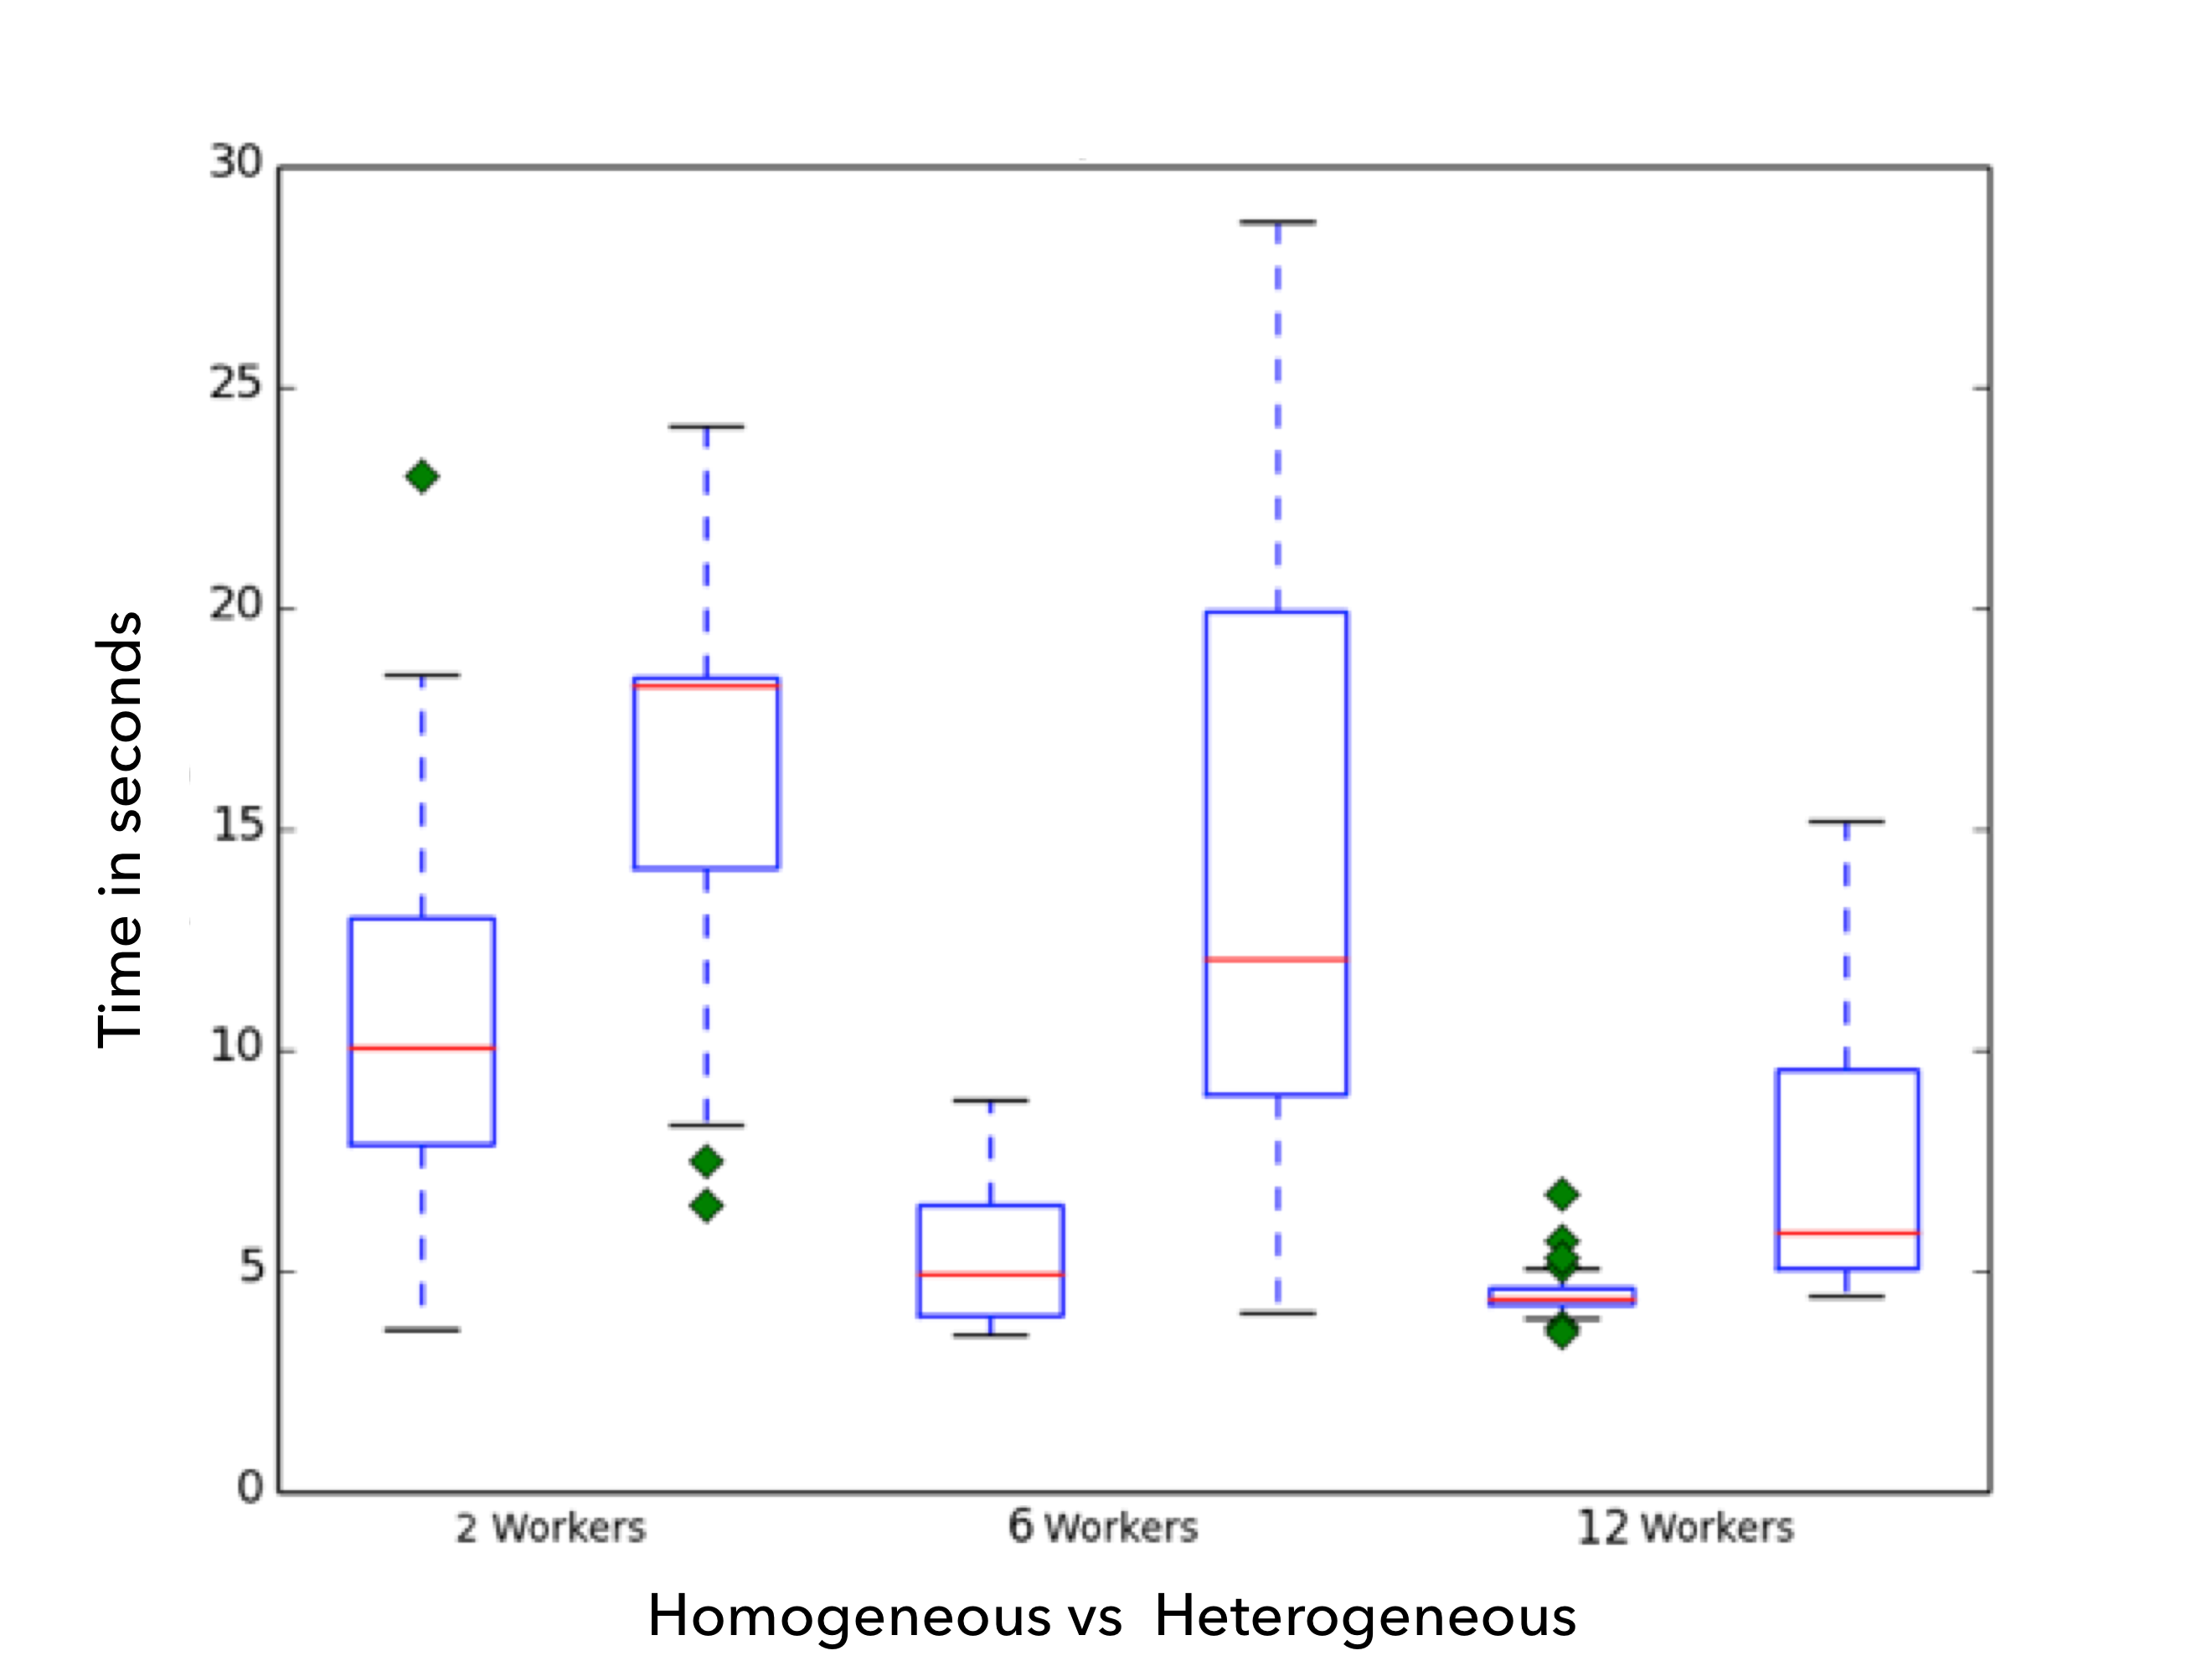
\includegraphics[width=10cm]{img/one_max_comp.png}
    \caption{Comparison of 30 runs of the 128 Bit OneMax problem. 
    Box-plot of the number of evaluations needed for solution, with a 2, 6 and 12 workers
    homogeneous configuration on the left side, and Heterogeneous configuration on the
    right side of each.
    }
    \label{fig:comp-onemax}
\end{figure*}

\section{Experiments}
 \label{sec:experiments}

The goal of this work is to determine if a random static parametrization for each of the $n$ EvoWorkers 
collaborating on a given run could achieve competitive results against an homogeneous tuned parametrization
\cite{fuku1,fuku2,garcia2014randomized}. The parameters considered to be randomly set for each EvoWorker 
where the crossover and mutation probabilities with a valid range of $[0,1]$. These parameters where 
selected because they effectively control which types of moves in the search space are
applied, and are related to the amount of exploration and exploitation
that is carried out. % \cite{}. Don't know if we need this - JJ
The other parameters and design choices used by EvoSpace and the EvoWorkers in our experiments are given in 
Table \ref{tab:params}. Additionally, for the binary OneMax problem bit-flip mutation
is used with an independent probability for each attribute to be flipped (indpb) of $0.05$, 
a two point crossover and a tournament selection of size 3. For the real-valued problems a Gaussian
mutation was applied with mu=$0$, sigma=$0.2$, and indpb=$0.05$; two point crossover and
a tournament selection of three. These values are kept static to measure only the effect of the 
parameters mentioned above.
    % Why do these parameters don't change?
    % Explained - Mario 



To measure the effectiveness of RPSS in EvoSpace two parametrization strategies are compared, 
similar to what is done in \cite{fuku1,fuku2,garcia2014randomized}. First, we consider the approach of setting all 
of the EvoWorker parameters homogeneously. In order to tune the homogeneous parameters,
we select the best configuration from 100 random parametrizations. 
Each of these random parametrization are evaluated based on their average performance over 10 
independent runs for each problem.
Hereafter, we refer to this method as the {\em homogeneous} configuration. Second, for RPSS the parametrizations
are not tuned, they are randomly generated for each EvoWorker, set independently at the beginning of each run.
Hereafter, we call this approach the {\em heterogeneous} configuration. Finally, we perform 30 independent runs
with both methods and report the average number of evaluations required by each strategy to find the
global optimum solution.

The algorithms are first evaluated using the OneMax (or BitCounting) problem proposed by 
Schaffer and Eshelman \cite{SE91}, this is a simple problem consisting in maximizing the number 
of ones of a bitstring. For the current experiments a 128 bit string was used. Since this
problem is not computationally demanding, more experiments where conducted for the tuning phase, 
tuning the parameters using 2, 6, and 12 EvoWorkers. Then, following \cite{fuku1}, 
five standard real-valued single objective optimization problems 
are used, these are the Rastrigin, Griewank, De Jong, Schaffer  and Ackley functions, 
with the number of dimensions set to 100 in each case. For these problems we use a real-valued vector
representation for each individual.


\begin{figure*}[t]
    \centering
    \subfigure  [6 workers]
    {
        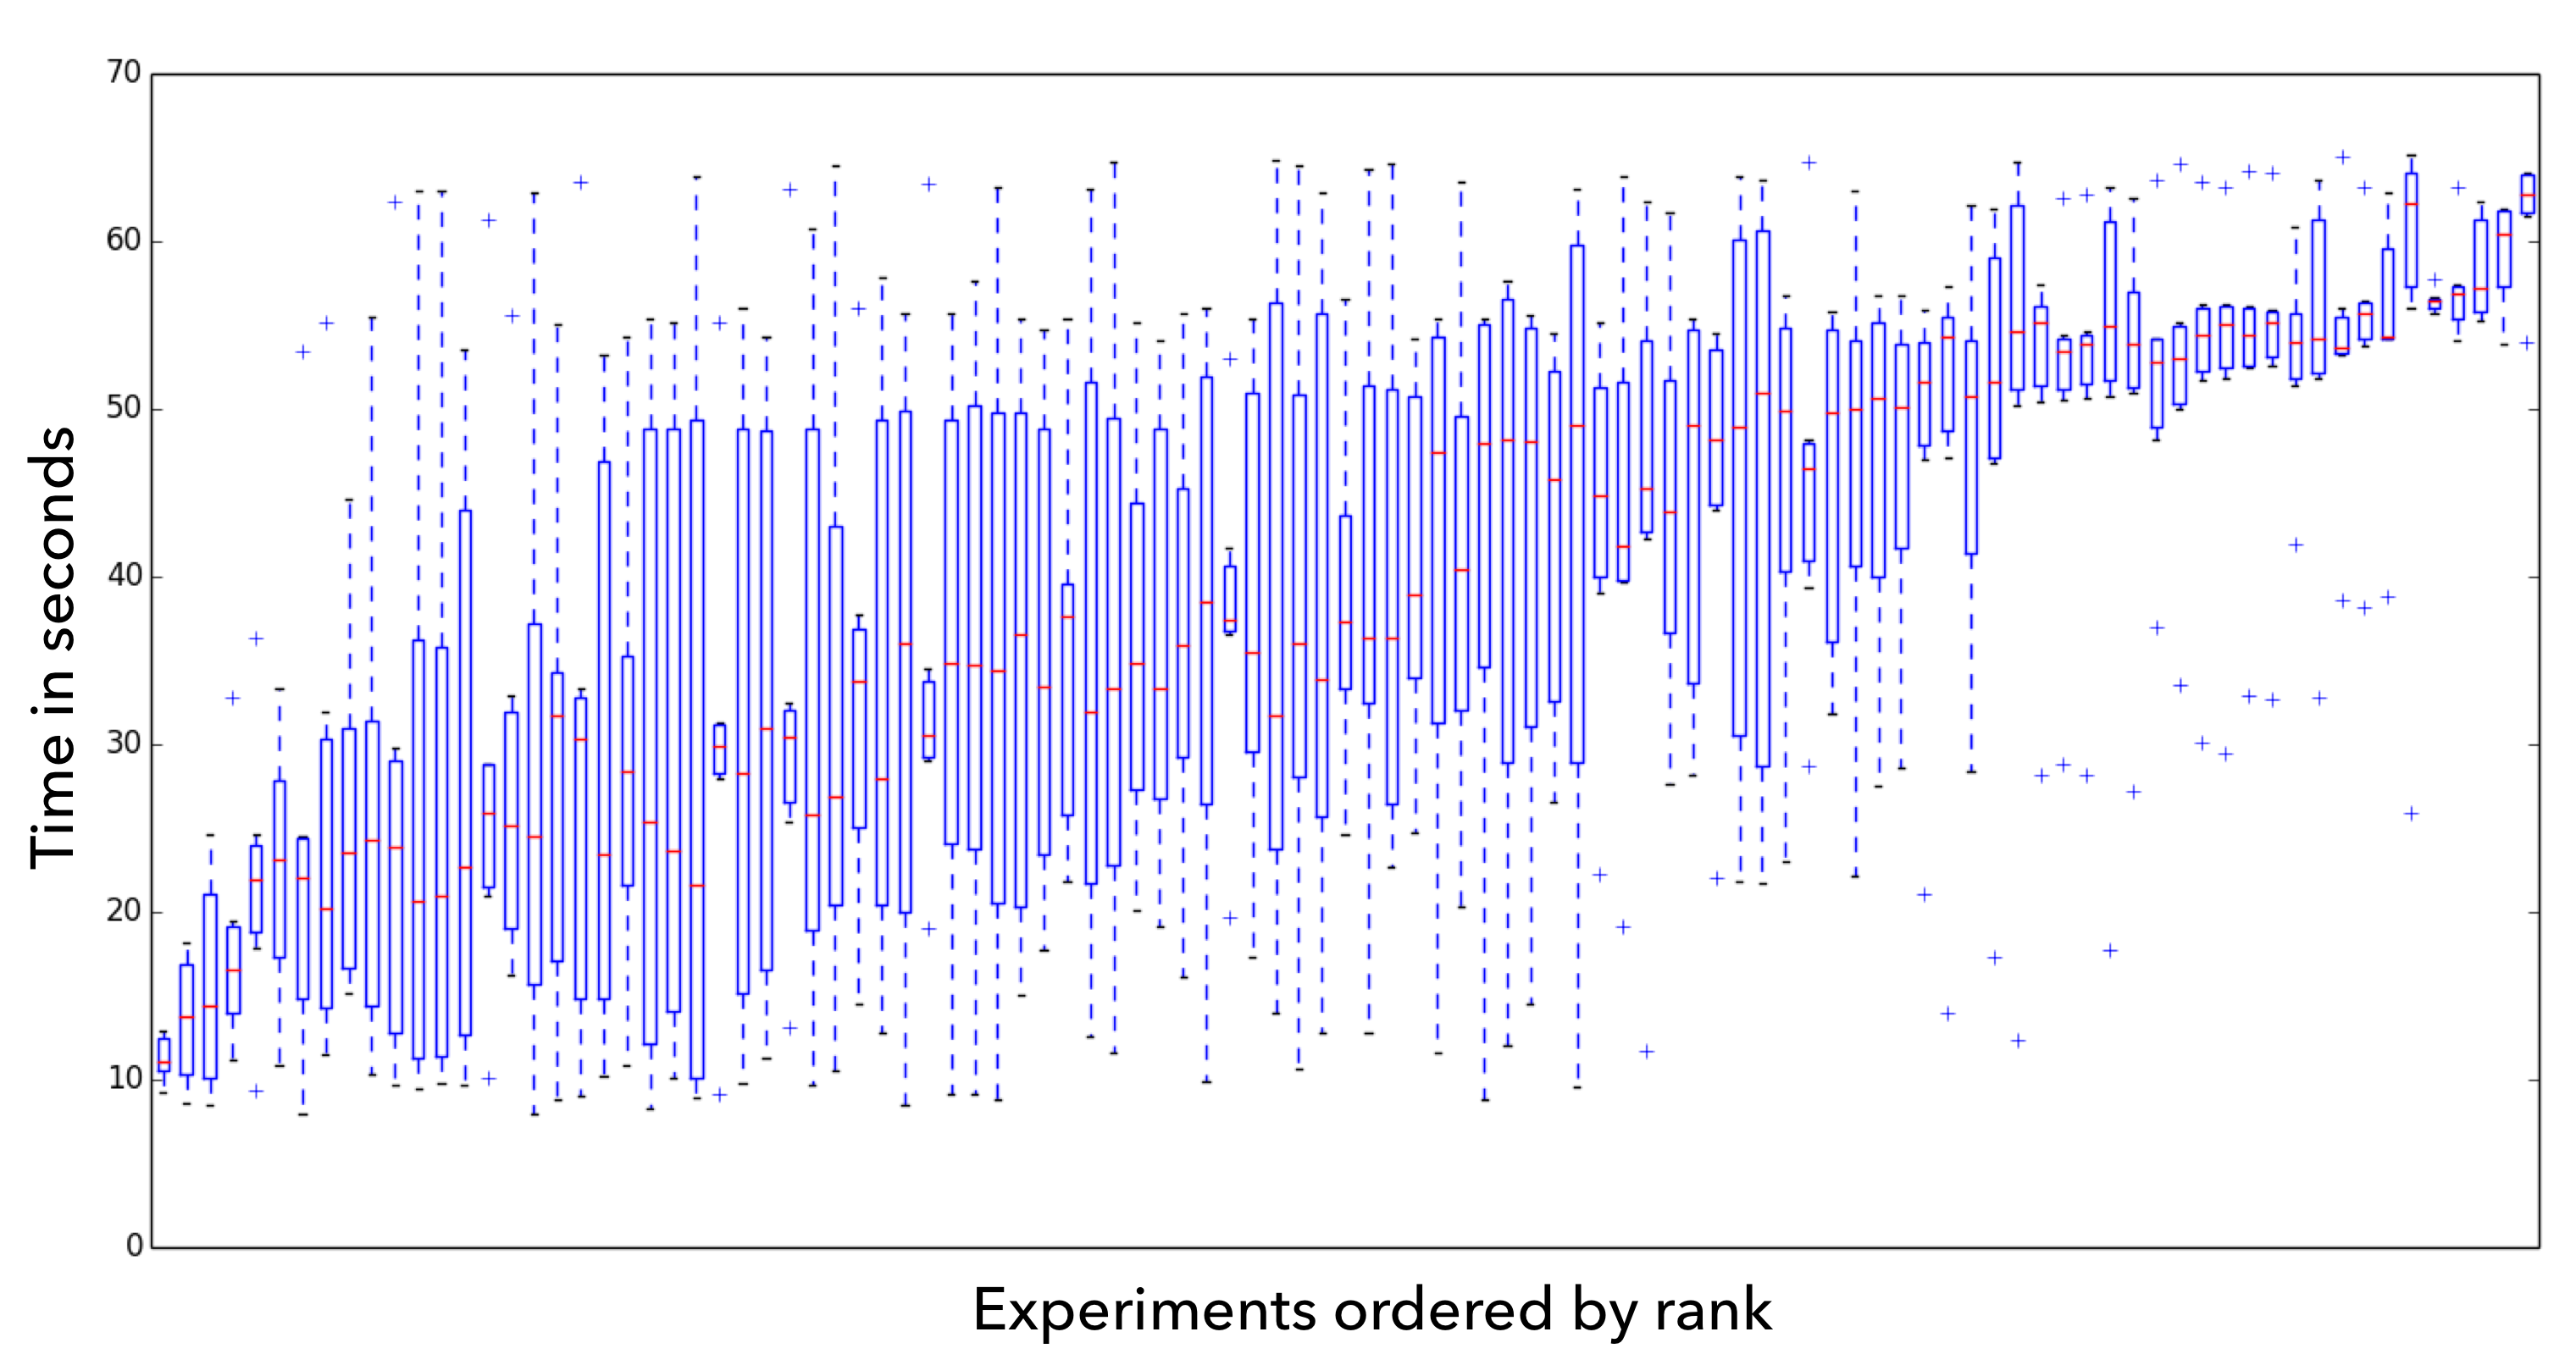
\includegraphics[width=2.2in]{img/6w_griewank_100_box.png}
    }
    \subfigure  [12 workers]
    {
        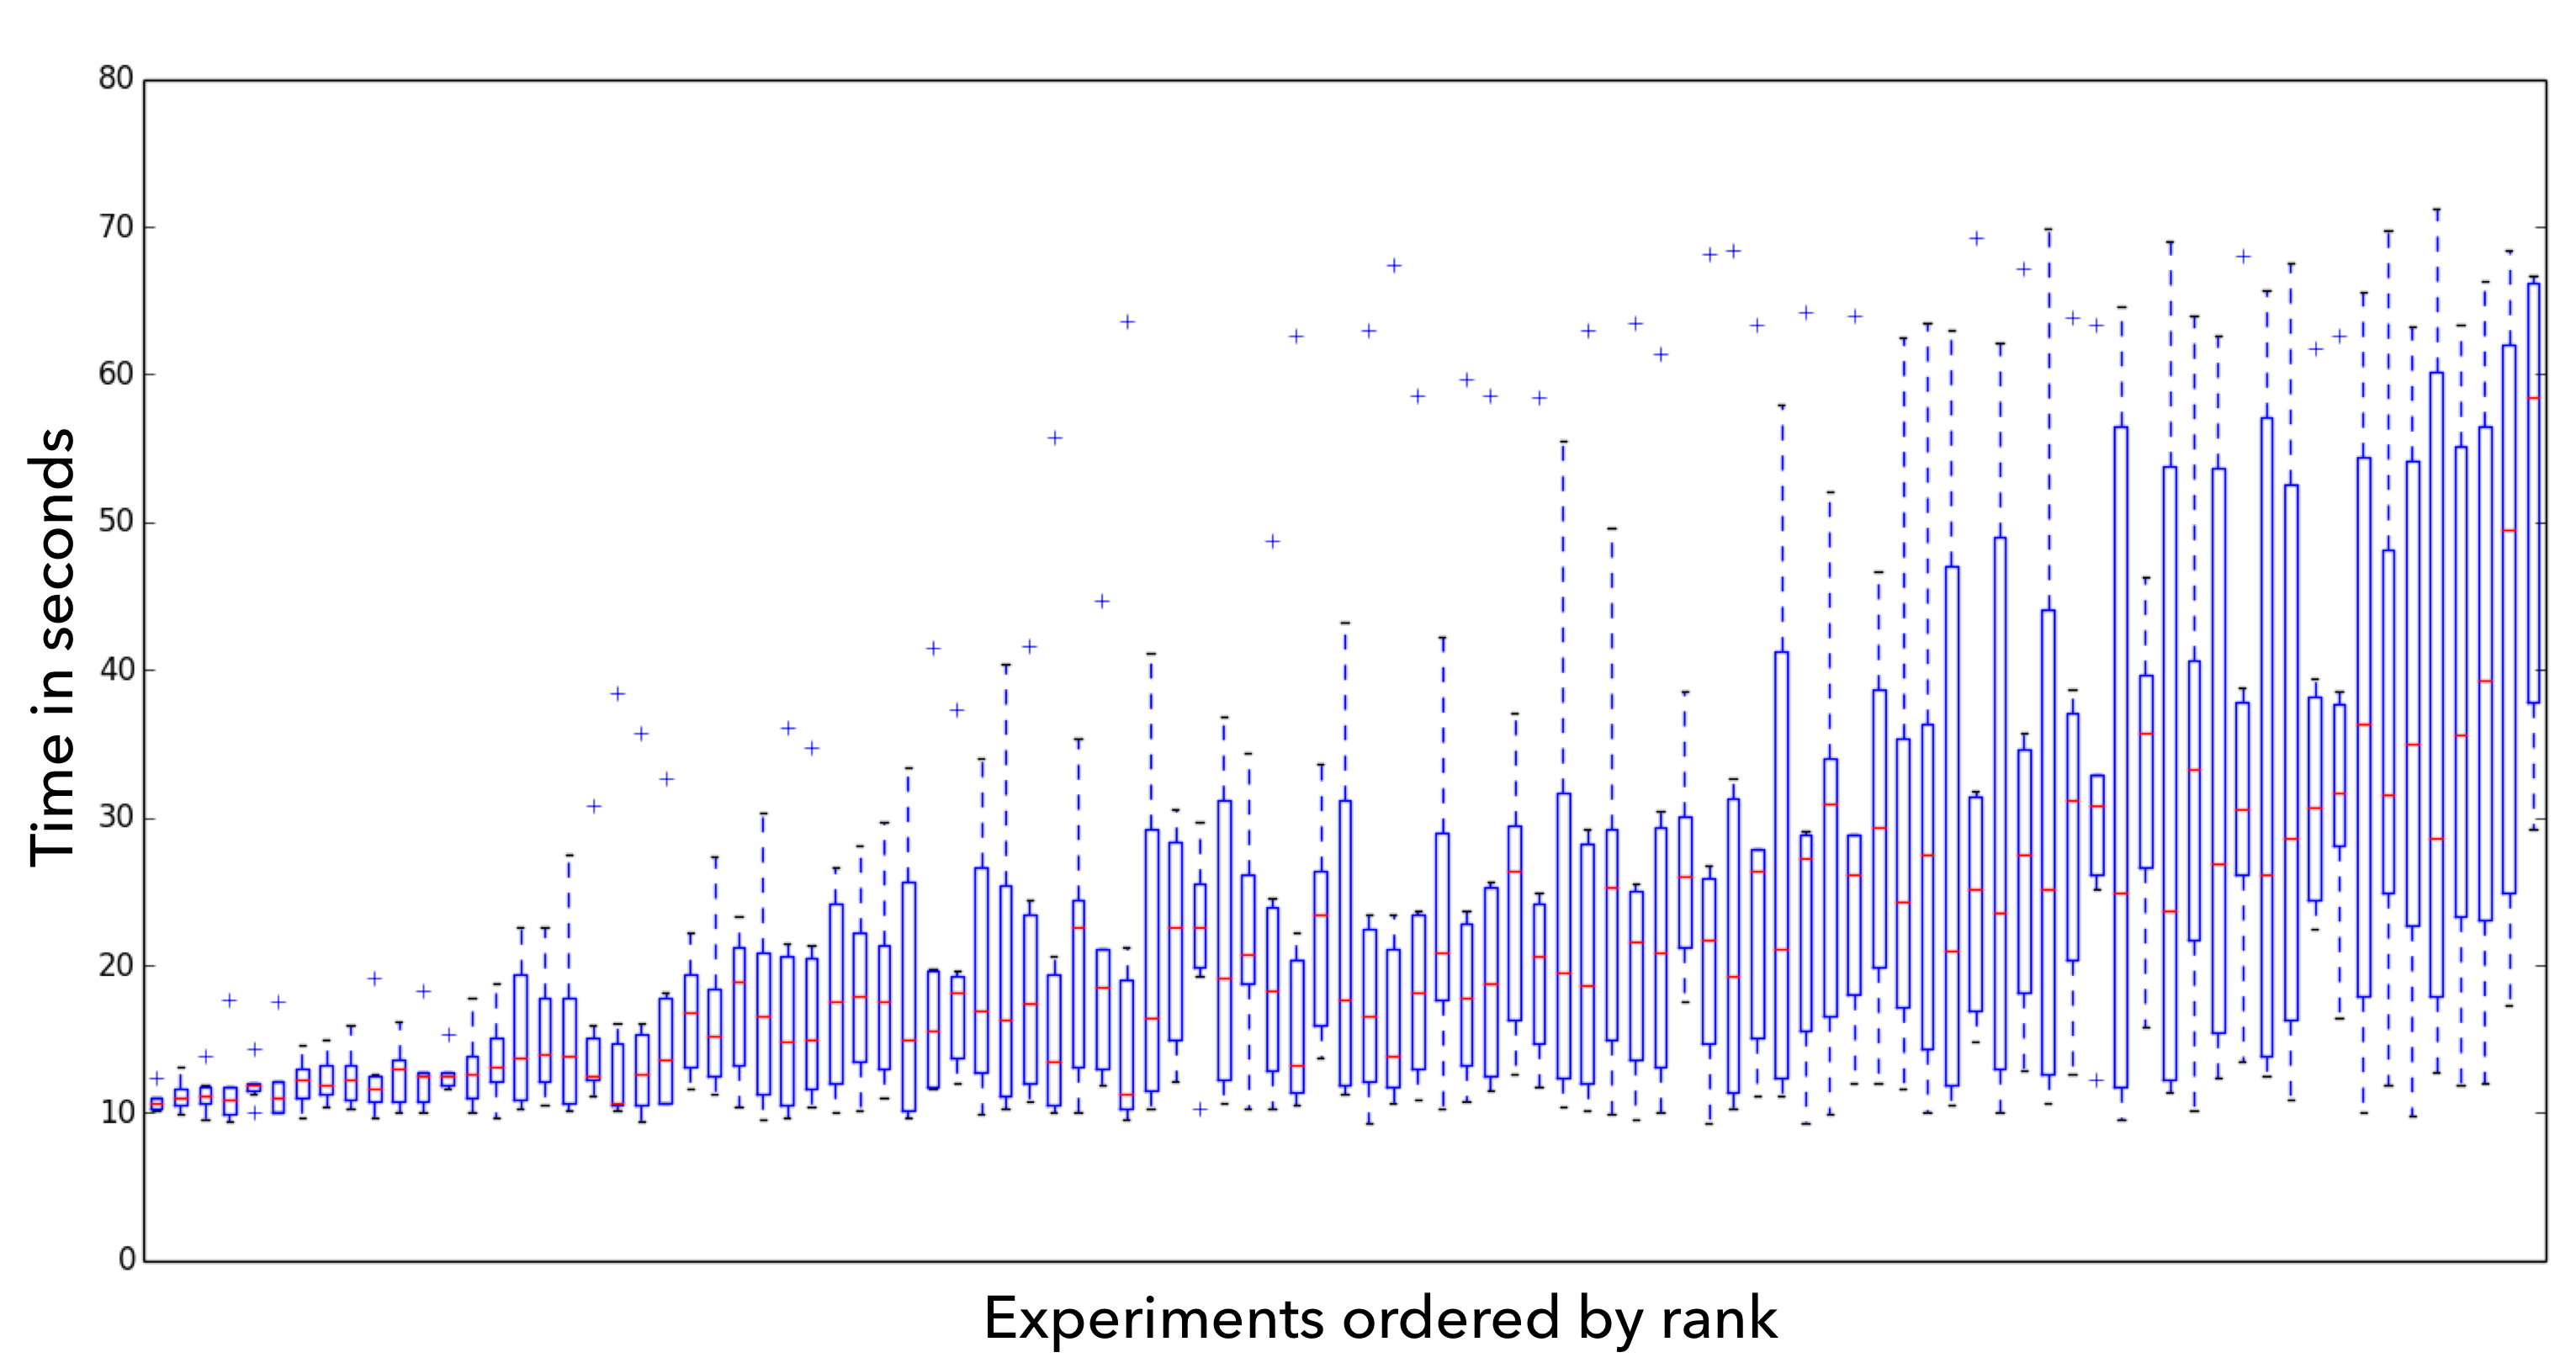
\includegraphics[width=2.2in]{img/12w_griewank_100_box.png}
    }

    \caption{100 experiments with random parameters for the 128 Bit Griewank 
    single-objective optimization test function. Experiments are ranked by 
    the mean time to solution of 5 runs, with (a) 6 workers, and (b) 12 workers.}
    \label{fig:griewank}
\end{figure*}


\begin{figure*}[t]
    \centering
    \subfigure  [Homogeneous]
    {
        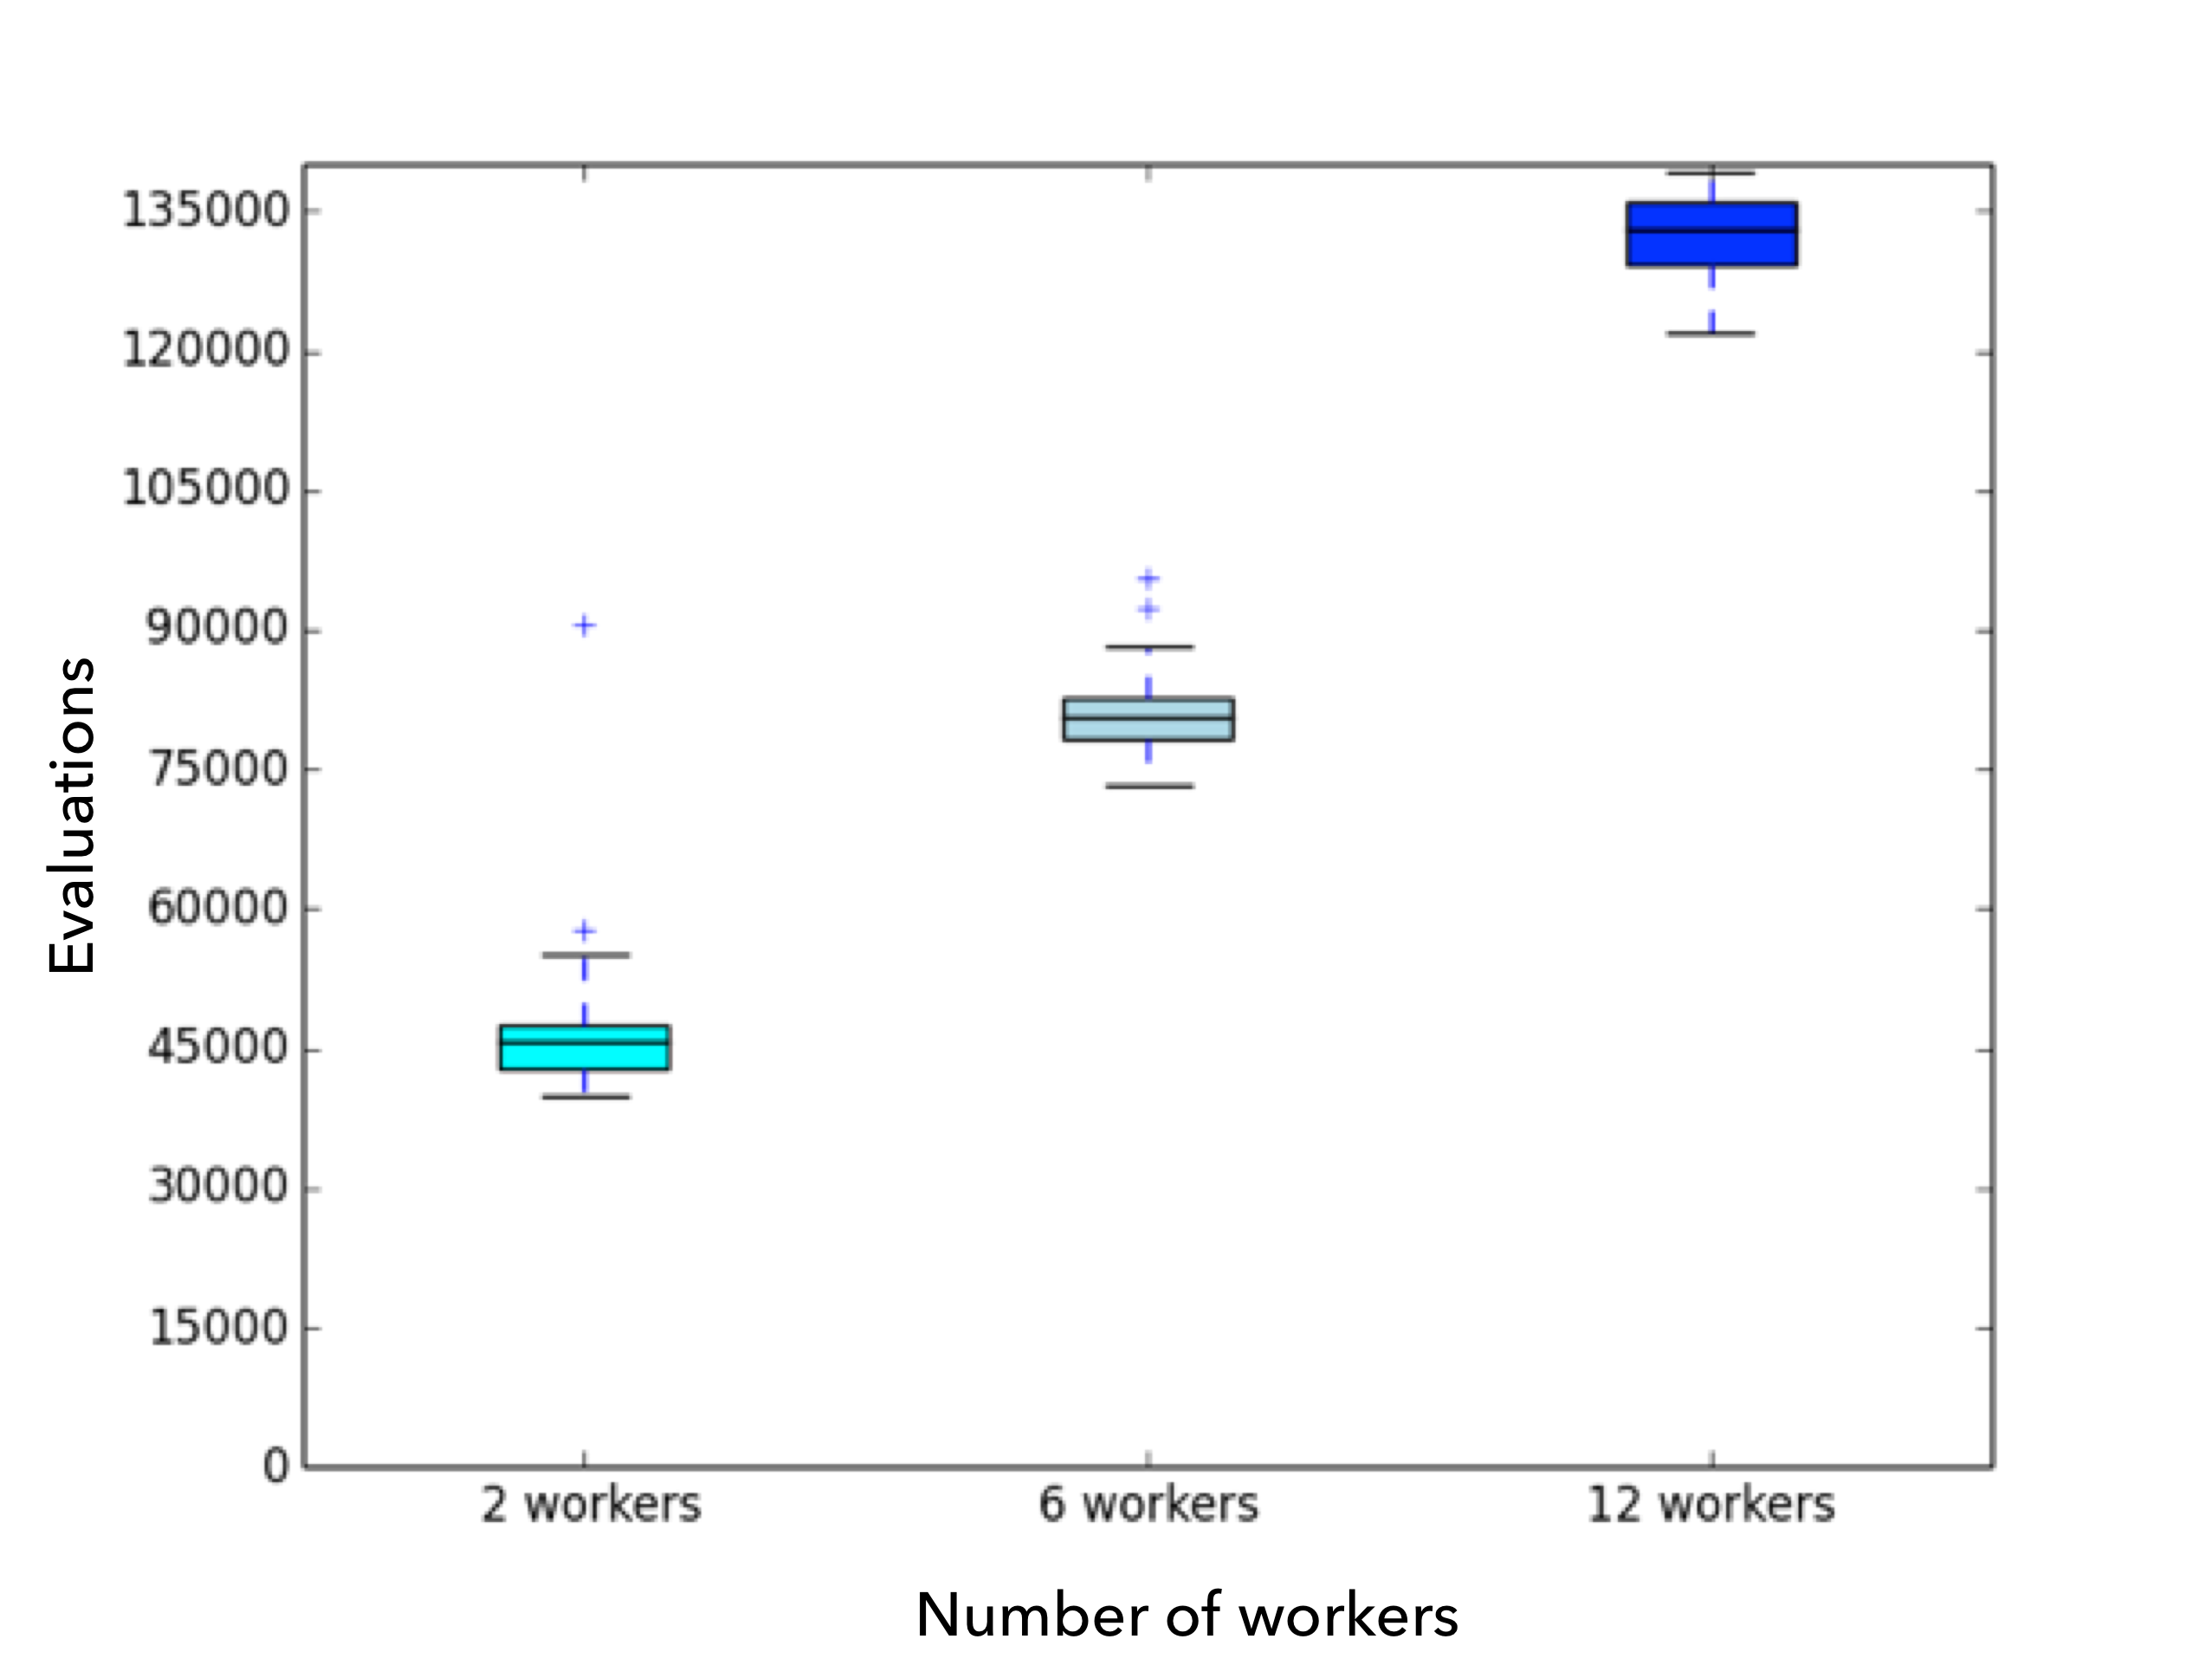
\includegraphics[width=2.2in]{img/griewank_evals_homo.png}
    }
    \subfigure  [Heterogeneous]
    {
        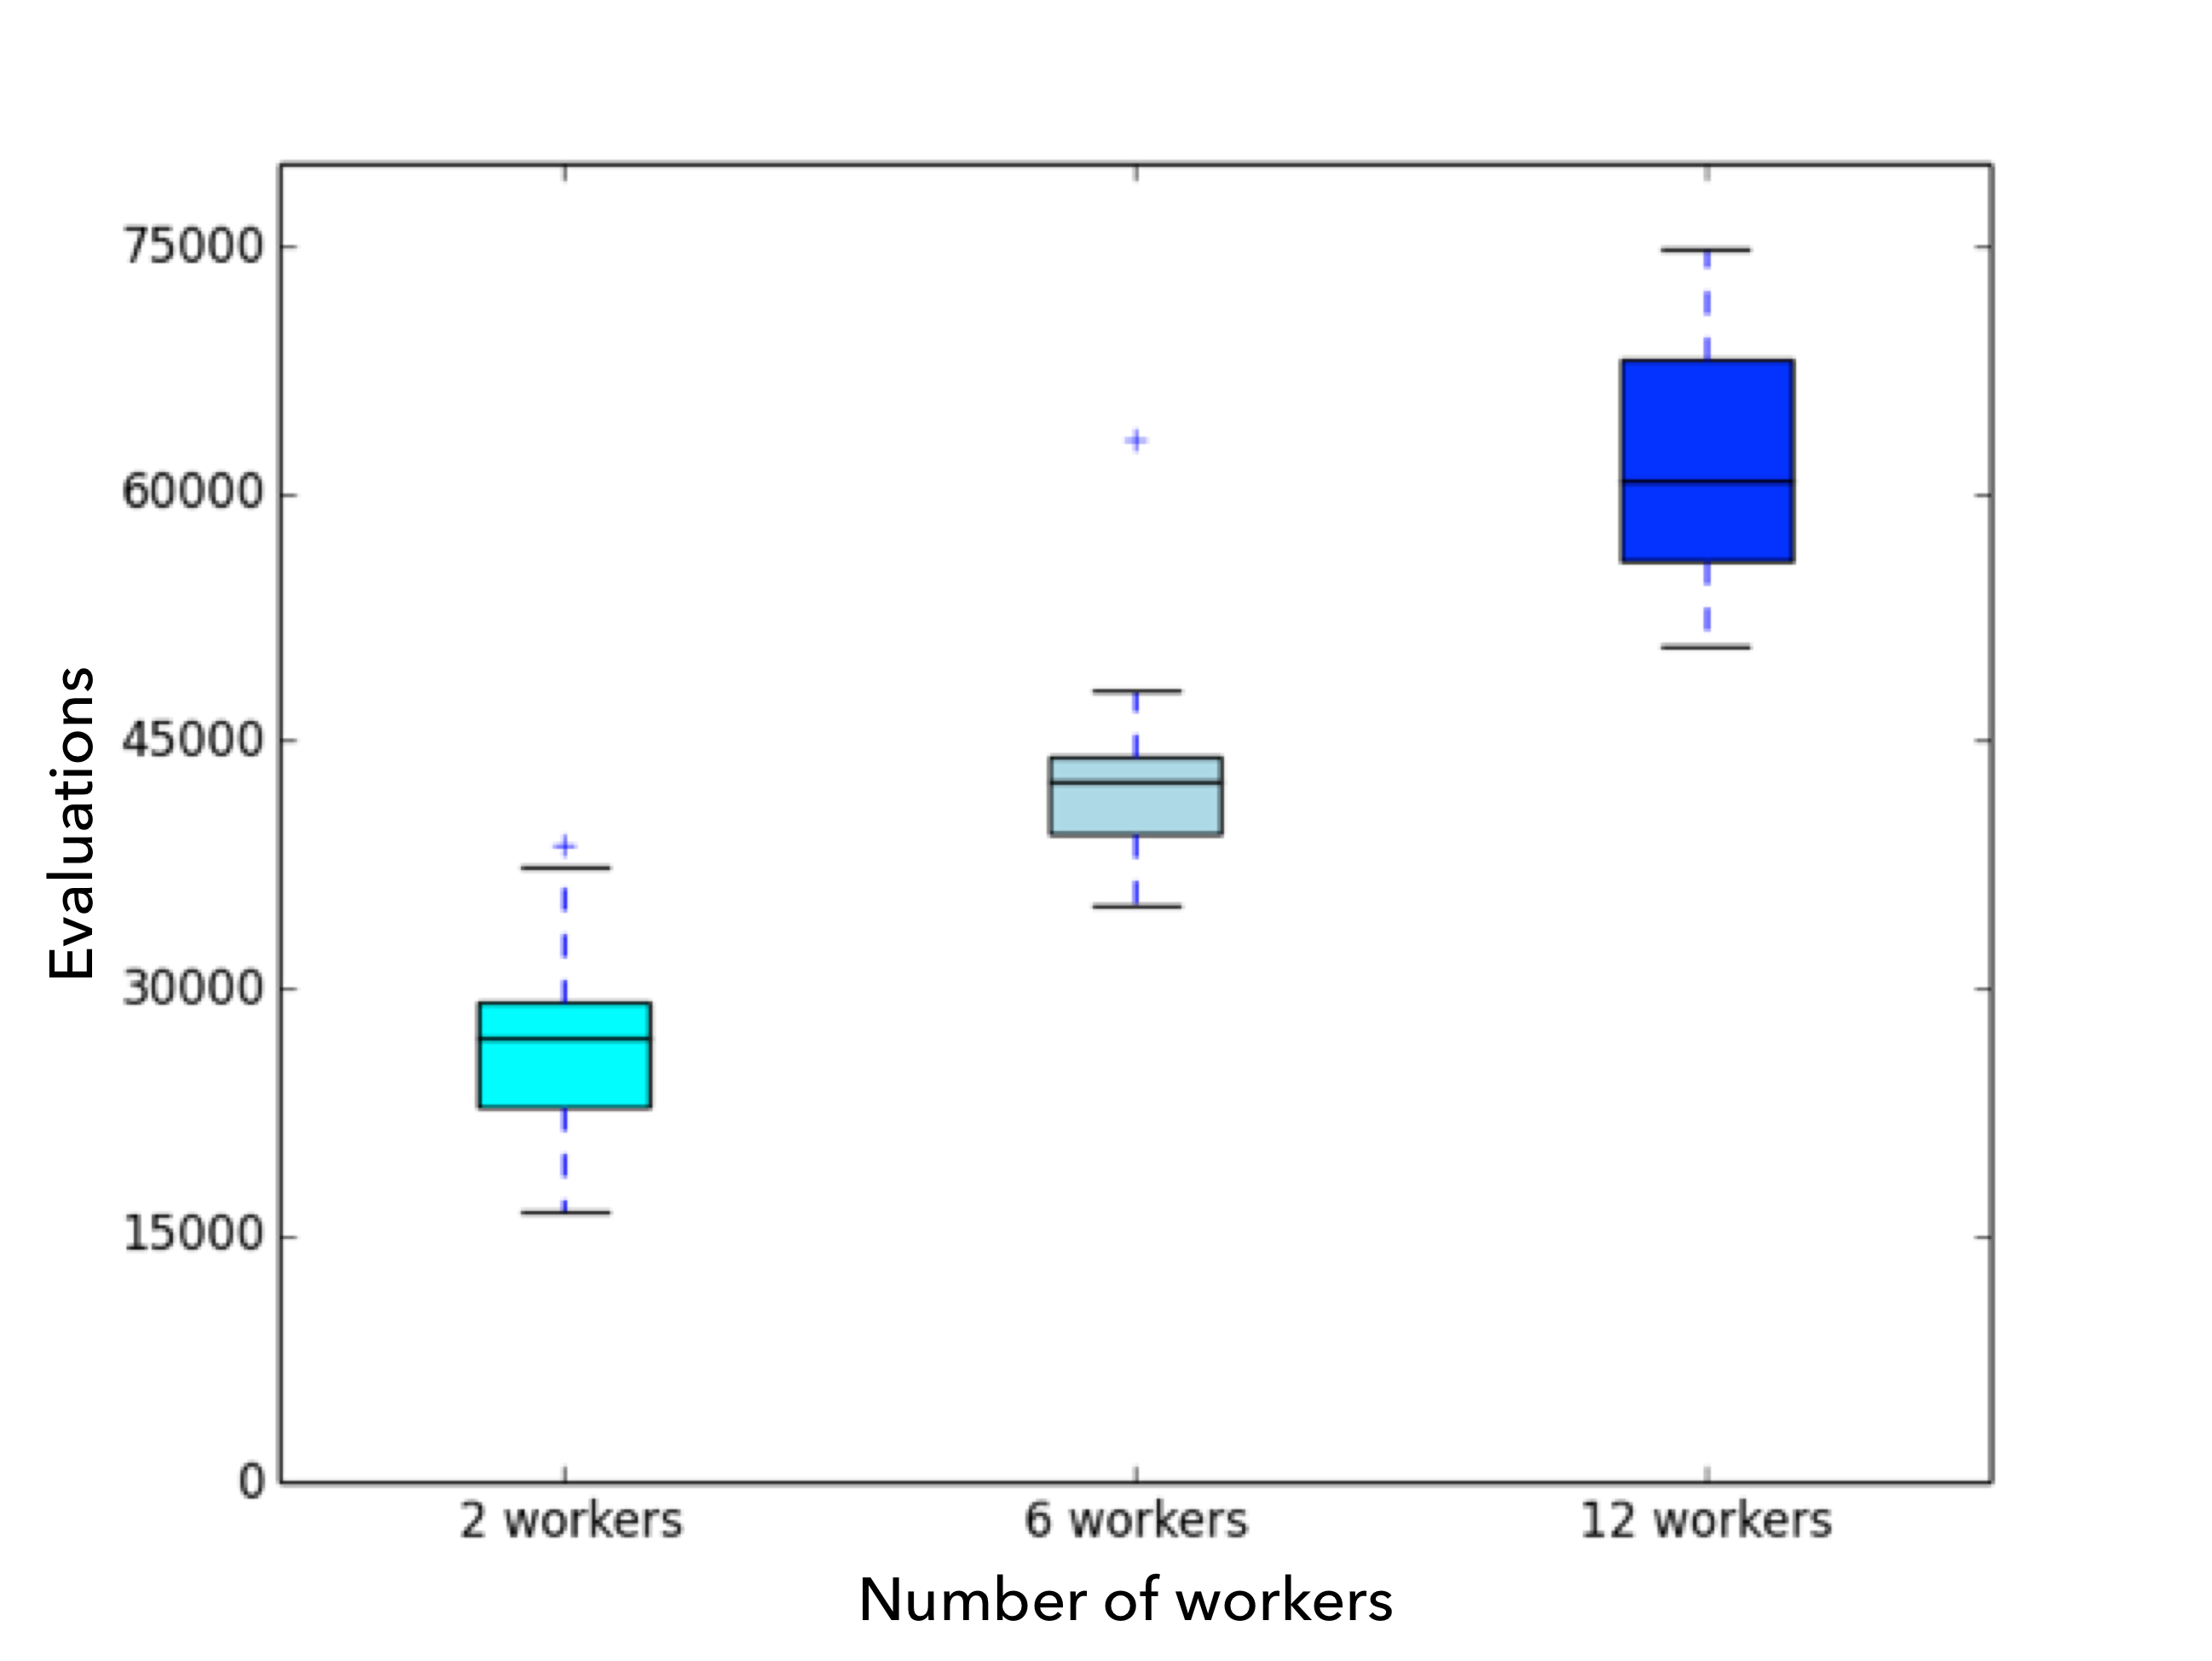
\includegraphics[width=2.2in]{img/griewank_evals_hetereo.png}
    }
      \caption{ 30 runs on the Griewank function. Box-plot of the number of evaluations needed for solution, 
                 with an (a) Homogeneous configuration, and (b) Heterogeneous configuration.}
    \label{fig:griewank-evals}
\end{figure*}

\begin{figure*}[t]
    \centering
    \subfigure  [Homogeneous]
    {
        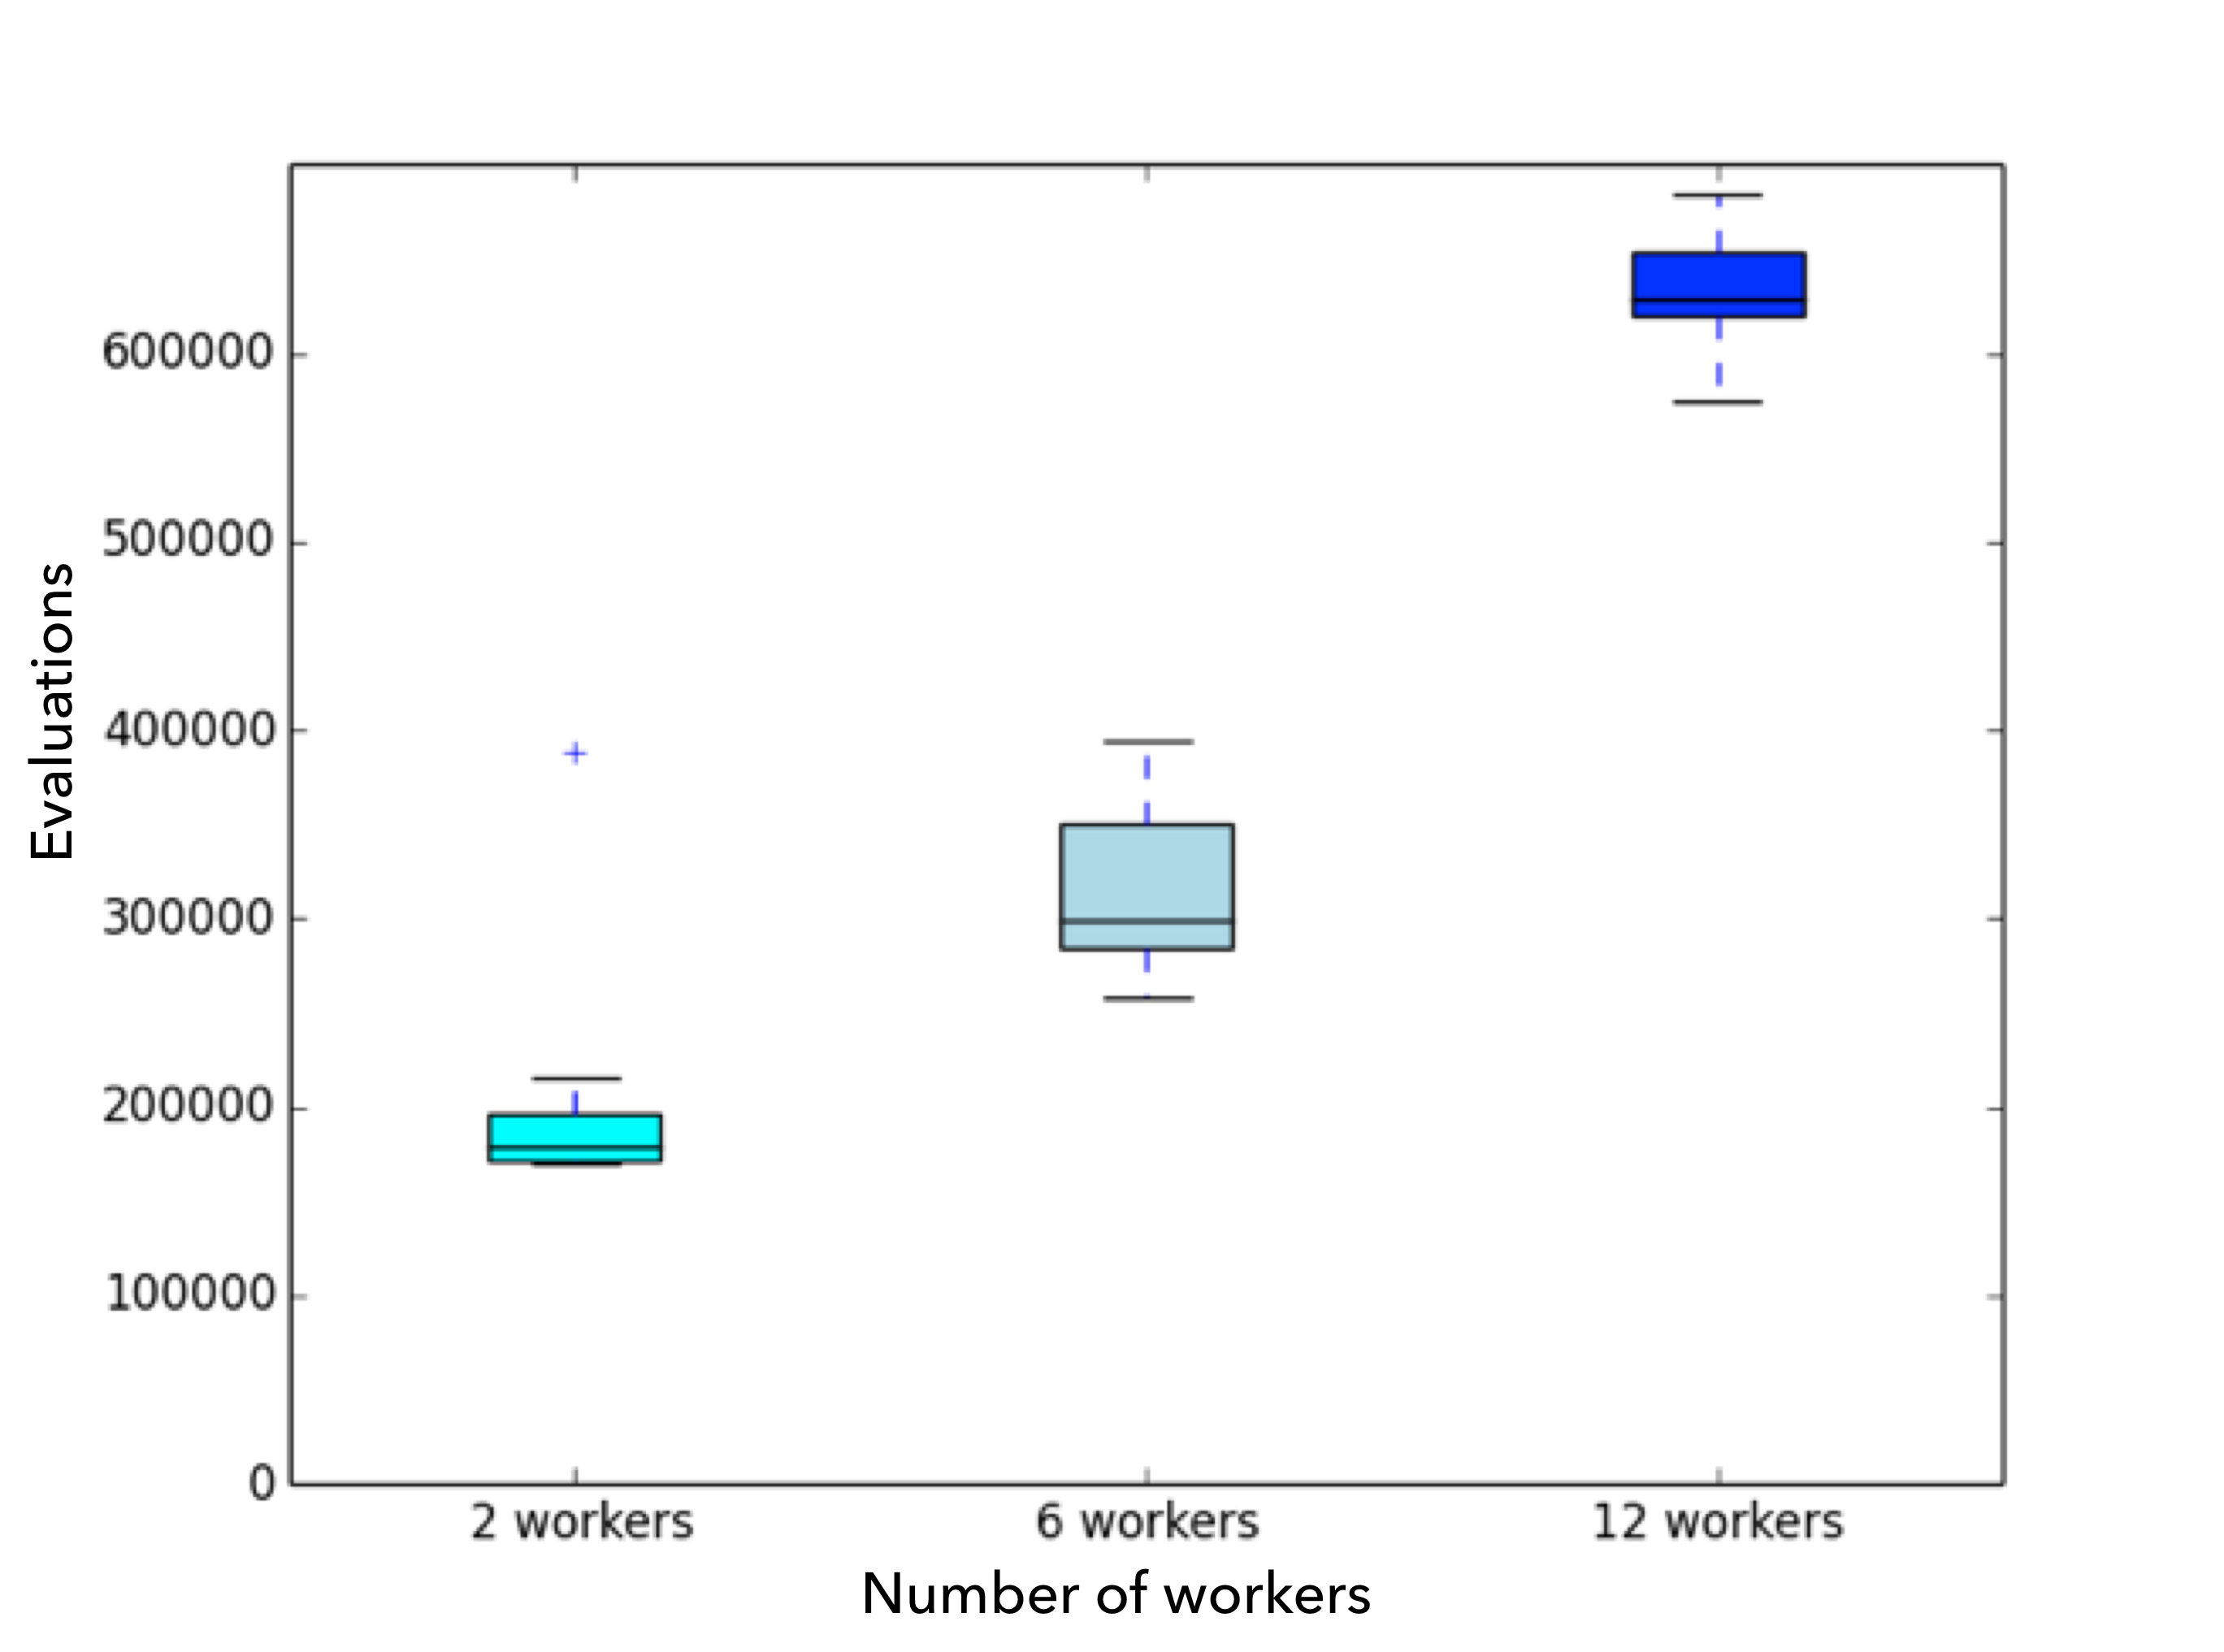
\includegraphics[width=2.2in]{img/schaffer_evals_homo.png}
    }
    \subfigure  [Heterogeneous]
    {
        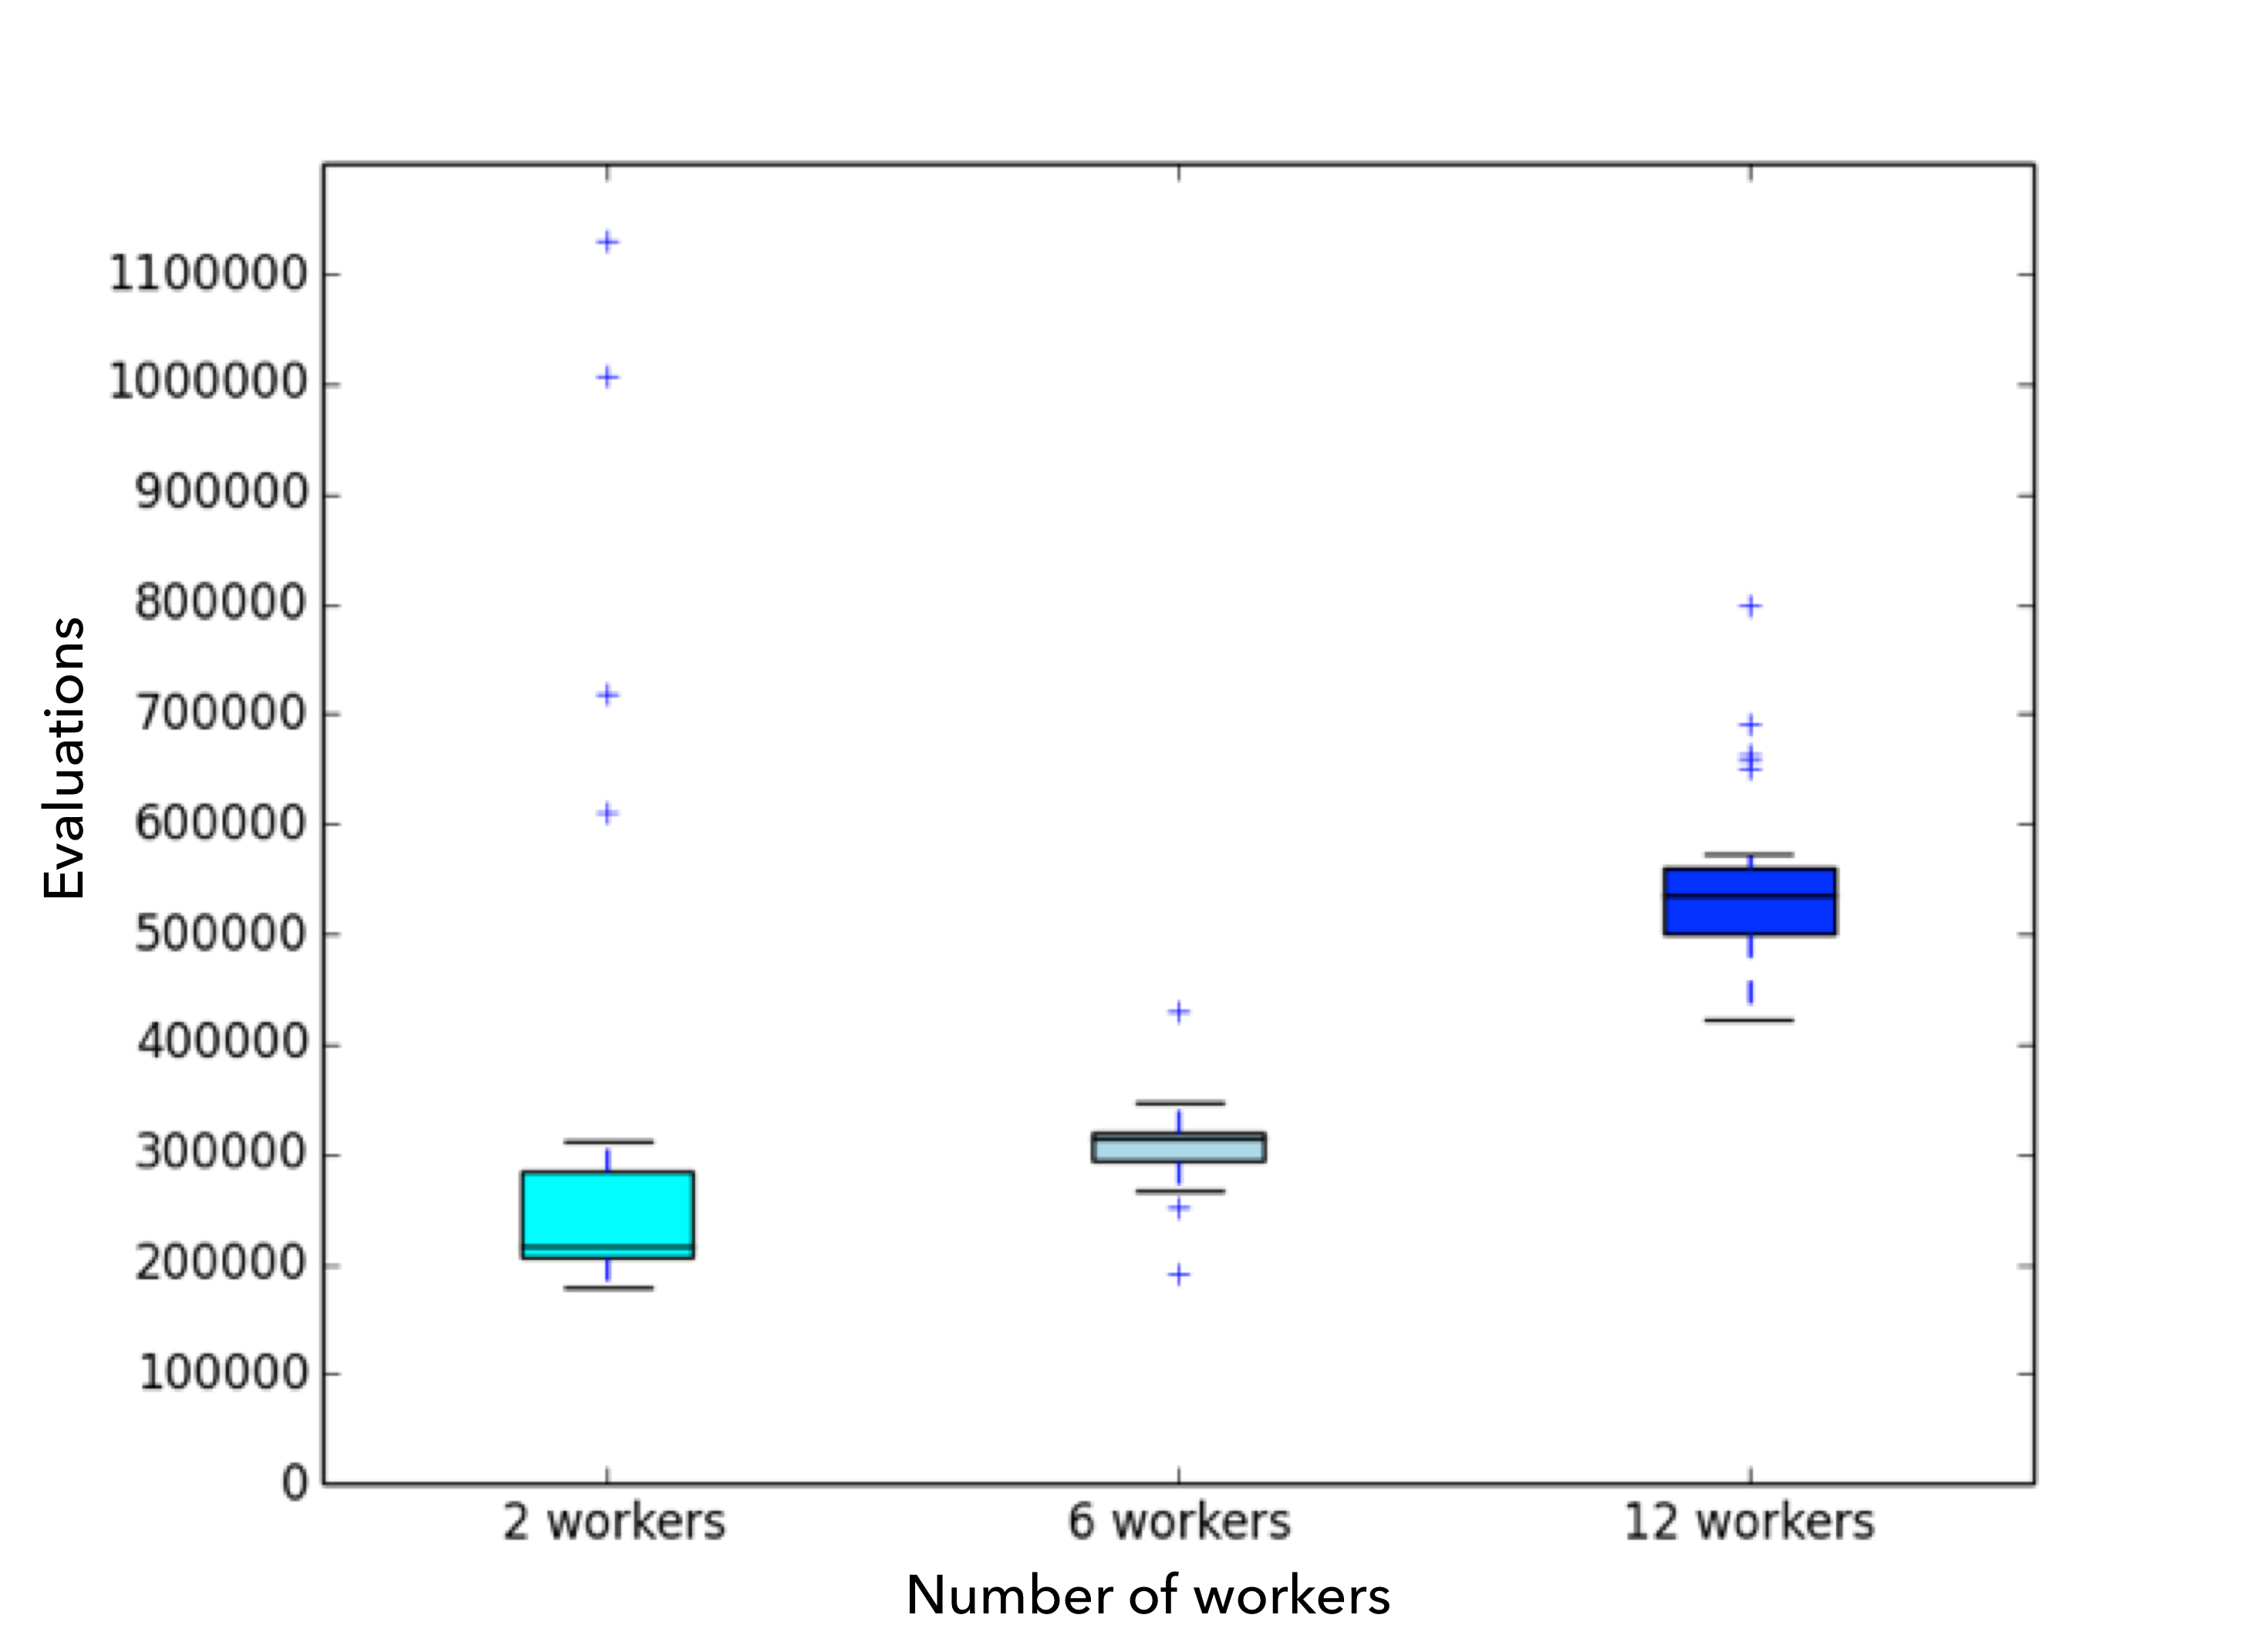
\includegraphics[width=2.2in]{img/schaffer_evals_hetereo.png}
    }
 

    \caption{30 runs on the Schaffer function. Box-plot of the number of evaluations needed for 
      solution, with an (a) Homogeneous configuration, and (b) Heterogeneous configuration.}
    \label{fig:schaffer}
\end{figure*}

\begin{figure*}[t]
    \centering
        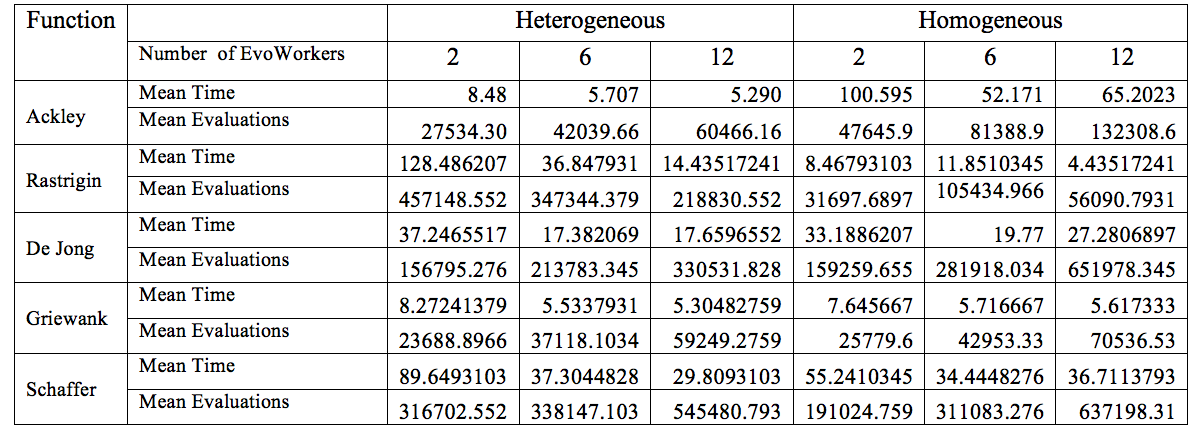
\includegraphics[width=4.5in]{img/table.png}
    \caption{Summary table of results. }
    \label{fig:summary}
\end{figure*}

\subsection{Results for OneMax}
As mentioned before, the first step is to simulate the manual tuning of the parameters 
by running 100 experiments with random parameters and then select the best configuration, 
using the median performance over 5 runs. Since the OneMax problem is solved by almost all
configurations, performance is determined by the time required to find the optimal solution.
%[FALTA ESPECIFICAR PORQUE SE USO EL TIEMPO AQUI, Y PORQUE EL NUMERO DE EVALUACIONES EN LOS OTROS EXPERIMENTOS]
Figure~\ref{fig:effort} shows the time required for different numbers of EvoWorkers. 
It can be observed that even with an homogeneous configuration, as the number of workers 
increases solutions are found faster. In general, increasing the number of workers increases 
the number of function evaluations carried out over a unit of time. This implies that the selection
of a good configuration could be found easier when using a higher number of workers, relative
to the total wall-clock time.  

In Figure~\ref{fig:comp-onemax} the results of 30 runs comparing against the RPSS approach is shown.
It can be observed that as the number of EvoWorkers increases the median of the time decreases, but
in this case the best of the heterogeneous solutions (12 workers) is only better than the worst homogeneous
solution. % Explain - JJ

\subsection{Results for Real-valued Optimization Functions}
The same steps as the previous section were followed when evaluating the five real valued 
optimization problems of this section.  For brevity only two representative functions are 
presented with figures, and summary of all the results are shown in Table~\ref{fig:summary}. As before
the first step is to tune the parameters for the homogeneous configuration.
In Figure \ref{fig:griewank}, the results of the tuning phase for 6 and 12 workers 
for the Griewank function are shown. For 12 workers results are not as flat as before, 
with times comparable to the 6 worker configuration in the best case.

To compare the performance of the homogeneous approach and the heterogeneous approach based on RPSS,
Figure \ref{fig:griewank-evals} compares the approaches based on the total number of function 
evaluations required to find the optimal solution.
%[SE DETIENE CUANDO SE ENCUENTRA EL OPTIMO, O CUANDO ESTAS CERCAS POR UN epsilon ?] 
% Optimo con hasta 7 decimas - Mario  
These results show a clear performance improvement, with the heterogeneous configuration 
reducing the total number of function evaluations required to find a solution,
independently of the number of workers used.
On the other hand, for the Schaffer function, performance is quite similar,
with the heterogeneous approach only providing a slight reduction in the number 
of function evaluations for the case with 12 EvoWorkers.
In the summary shown in Table~\ref{fig:summary} two extreme cases are found, the Ackley and Rastrigin functions.
In the former, the heterogeneous configuration achieves the best performance, while the opposite is true on the latter.
Finally, performance on the De Jong function also favors the heterogeneous configurations.

\section{Conclusions and Further Work}
\label{sec:conclusions}
This paper presents an evaluation of the RPSS parametrization approach on 
a pool-based EA, using the OneMax problem and five test functions. 
Using the RPSS approach, it seems that a PEA can be executed successfully 
without any form of parameter tuning, achieving comparable results to standard homogeneous
parametrizations. Results also show that the benefits of a RPSS are not only present
when using a heterogeneous approach, even a random homogeneous configuration could bring
benefits. Unfortunately the RPSS strategy is not a silver bullet, as there are cases
when is the best approach. Future work will focus on using other EA techniques, 
such as genetic programming or particle swarm optimization for having more heterogeneous
workers, the RPSS could be use in those cases where each algorithm has different sets of
parameters. Another interesting line of work is the dynamic adaptation of parameters by
measuring the diversity of each worker or returned sample.   

\section*{Acknowledgments}

This work has been supported in part by:  Ministerio espa\~{n}ol de
Econom\'{\i}a y Competitividad under project TIN2014-56494-C4-3-P
(UGR-EPHEMECH).


\bibliographystyle{abbrv}
\bibliography{../../bib/biblio,../../bib/evospace-i,../../bib/parameters,../../bib/volunteer,../../bib/geneura}

\end{document}
